% Fuse: a per-stream reliable transport over UDP -- project report (CS3530: Computer Networks)
% Build:  latexmk -pdf report.tex      (or: pdflatex report.tex, run three times)
\documentclass[11pt,a4paper,oneside]{report}

\usepackage[T1]{fontenc}
\usepackage[utf8]{inputenc}
\usepackage{lmodern}
\usepackage{microtype}
\usepackage[a4paper,margin=2.5cm]{geometry}
\usepackage{amsmath,amssymb}
\usepackage{array,booktabs,tabularx,longtable,multirow}
\usepackage{xltabular}
\usepackage{enumitem}
\usepackage[table]{xcolor}
\usepackage{caption}
\usepackage{float}
\usepackage{listings}
\usepackage{tikz}
\usetikzlibrary{arrows.meta,positioning,shapes.geometric,shapes.multipart,fit,calc,automata,backgrounds,decorations.pathreplacing}
\usepackage{fancyhdr}
\usepackage{titlesec}
\usepackage[hidelinks]{hyperref}

\setlist{itemsep=2pt,topsep=4pt}
\setlength{\parskip}{3pt}
\setlength{\emergencystretch}{3em}
\captionsetup{font=small,labelfont=bf}
\renewcommand{\arraystretch}{1.15}

\definecolor{codebg}{RGB}{246,247,249}
\lstset{basicstyle=\ttfamily\small,backgroundcolor=\color{codebg},frame=single,rulecolor=\color{black!15},
        columns=fullflexible,keepspaces=true,breaklines=true,showstringspaces=false,
        xleftmargin=4pt,xrightmargin=4pt,aboveskip=6pt,belowskip=6pt}

\usepackage{url}
\makeatletter\g@addto@macro\UrlBreaks{\do\_\do\:\do\]\do\,}\makeatother
\DeclareUrlCommand\code{\urlstyle{tt}}
\newcommand{\fitwidth}[1]{\resizebox{\ifdim\width>\linewidth\linewidth\else\width\fi}{!}{#1}}
\newcommand{\vviii}{\textsuperscript{(v8)}}

\titleformat{\chapter}[hang]{\normalfont\huge\bfseries}{\thechapter.}{0.6em}{}
\titlespacing*{\chapter}{0pt}{-10pt}{18pt}

\pagestyle{fancy}
\fancyhf{}
\fancyhead[L]{\small\nouppercase{\leftmark}}
\fancyhead[R]{\small Fuse: a per-stream transport over UDP}
\fancyfoot[C]{\small\thepage}
\renewcommand{\headrulewidth}{0.4pt}
\fancypagestyle{plain}{\fancyhf{}\fancyfoot[C]{\small\thepage}\renewcommand{\headrulewidth}{0pt}}

% TikZ styles shared by the figures
\tikzset{
  box/.style={draw,rounded corners=2pt,align=center,font=\small,inner sep=4pt,fill=white},
  core/.style={box,fill=blue!6},
  api/.style={box,fill=green!8},
  io/.style={box,fill=orange!10},
  arr/.style={-{Stealth[length=2.2mm]},thick},
  msg/.style={-{Stealth[length=2mm]},semithick},
  st/.style={draw,rounded corners=6pt,align=center,font=\small,minimum height=7mm,inner sep=3pt,fill=blue!5},
  lbl/.style={font=\footnotesize,align=center},
}

\begin{document}

\begin{titlepage}
  \centering
  \vspace*{3cm}
  {\Huge\bfseries Fuse: A Per-Stream Reliable\\[4pt] Transport Protocol over UDP\par}
  \vspace{0.8cm}
  {\Large Design, Implementation, Security Hardening and Evaluation\\ of Protocol Version 8\par}
  \vspace{2.2cm}
  {\large Project Report\par}
  \vspace{0.4cm}
  {\large CS3530: Computer Networks\par}
  \vspace{2.2cm}
  {\large
  \begin{tabular}{c}
    Boreddy Sri Sai Abhinav Reddy\\[3pt]
    Chiruvella Gagan Chandra Sai Ram\\[3pt]
    Kamal Koushik Duppalapadi\\[3pt]
    Tavva Dinesh Reddy
  \end{tabular}\par}
  \vfill
  {\small Source code: \code{https://github.com/kamalkoushikd/fuse-nw} (protocol version 8, commit \code{9706e21})\par}
\end{titlepage}

\pagenumbering{roman}
\begin{abstract}
\noindent
Applications that carry a mixture of loss-tolerant, latency-sensitive data and loss-intolerant,
correctness-sensitive data over one session are served poorly by the standard transports. TCP serialises all of
it behind a single ordered byte stream and a single congestion window, so one lost segment delays everything that
follows. QUIC removes head-of-line blocking between streams but keeps congestion control connection-wide and
makes TLS mandatory. This report describes \emph{Fuse}, a datagram transport built directly on UDP in which every
stream owns its own sequence space, receive window, retransmission store and congestion controller, and in which
reliability, ordering and coalescing are per-stream properties.

We describe the wire format, the reliability core (a ring-indexed selective-acknowledgement window with
reorder-tolerant negative acknowledgements), per-stream congestion control with slow start, RFC~6298
retransmission timers and pacing, and three transports built on these pieces: a sharded, GSO-batched bulk
transfer with resumable file reception, a message-oriented socket-style C API, and a multiplexed transfer
serviced by an autoscaling worker pool. A full security and correctness review of the earlier version found 31
problems. We present protocol version~8, which fixes every one outside the socket-style SDK and the HTTP
mapping. Among the fixes are an AES-GCM nonce-reuse flaw on retransmission, an unauthenticated control plane,
missing address and path validation, missing flow control, and an unused selective-acknowledgement bitmask.

All 206 tests pass (184 without the cryptographic backend). Under emulated packet loss, version~8 transfers 2.7
times faster at 2\% loss and 4.4 times faster at 5\% loss than version~7, with byte-identical output in every
experiment, and without loss of loopback throughput. We close with the limitations that remain and the work
needed to address them.
\end{abstract}

\tableofcontents
\listoffigures
\listoftables

\clearpage
\pagenumbering{arabic}

\chapter{Introduction}\label{ch:intro}

\section{Problem statement}

Many networked applications send two kinds of data at the same time. The first kind is \emph{loss-tolerant and
latency-sensitive}: telemetry samples, media frames, game or robot state, position updates. For this data a
newer value supersedes an older one, and waiting for the retransmission of a lost packet is worse than simply
skipping it. The second kind is \emph{loss-intolerant and correctness-sensitive}: files, configuration, logs,
commands. Here every byte must arrive, and arrive intact, but small delays are acceptable.

When both kinds share one transport connection, the transport must make the right trade-off for each of them
independently. The two standard choices cannot do this:

\begin{itemize}
  \item \textbf{TCP}~\cite{rfc9293} provides one ordered byte stream per connection. A single lost segment holds
    back every byte behind it until it is retransmitted (\emph{head-of-line blocking}). All data on the
    connection also shares one congestion window, so a loss in the bulk transfer slows the latency-sensitive
    traffic too. Opening several TCP connections avoids the blocking but multiplies handshakes and offers no
    shared session.
  \item \textbf{QUIC}~\cite{rfc9000,quic-design} multiplexes independent streams over UDP, so a loss on one
    stream no longer blocks another. Its congestion control is still defined per connection~\cite{rfc9002}, so
    the streams still compete for one window. It also makes TLS~1.3 mandatory~\cite{rfc9001}, which is a fixed
    cost even on a trusted link, and unreliable delivery is a separate extension rather than a property of a
    stream.
\end{itemize}

\noindent The problem this project addresses is therefore:

\begin{quote}
\emph{Design and build a transport protocol over UDP in which reliability, ordering and congestion control are
properties of each individual stream rather than of the connection, so that loss-tolerant and loss-intolerant
traffic can share one session without either one degrading the other. The protocol must remain fast enough for
bulk data and secure enough to be used on untrusted networks.}
\end{quote}

\section{Approach in brief}

Fuse is a datagram transport built directly on UDP. Every stream has its own sequence-number space, its own
receive window, its own retransmission store and its own congestion controller. Three per-stream flags,
negotiated when a session is set up, decide how the stream behaves:
\begin{itemize}
  \item \code{LOSSLESS} decides whether missing blocks are retransmitted;
  \item \code{ORDERED} decides whether blocks are delivered in sequence or as soon as they arrive;
  \item \code{COALESCE} decides whether a full send queue drops its oldest entry or makes the producer wait.
\end{itemize}

Encryption is optional and configured locally: when both ends hold the same pre-shared key, every block is
sealed with AES-256-GCM and, since version~8, every control message is authenticated. Throughput comes from
batched system calls (UDP generic segmentation offload and \code{recvmmsg}~\cite{gso,recvmmsg}), fixed-size
storage with no allocation on the per-packet path, and per-lane parallel encryption.

On top of a common core of building blocks, the repository offers three transports:
\begin{itemize}
  \item a sharded bulk transfer for buffers and files, with resumable file reception;
  \item a socket-style, message-oriented C API;
  \item a multiplexed transfer that services many streams with an autoscaling pool of worker threads.
\end{itemize}

\section{Contributions of this work}

The protocol existed at version~7 when this work began. Our contributions are:

\begin{enumerate}
  \item \textbf{A complete study of the design and implementation.} We read the entire repository and document
    the wire format, every building block, the three transports, their state machines and the engineering
    principles they follow (Chapters~\ref{ch:arch}--\ref{ch:sdkmux}).
  \item \textbf{A security and correctness hardening of the protocol core, released as protocol version~8.} A
    review of version~7 found 31 issues. We fixed every one of them in the protocol core, deliberately leaving
    the socket-style SDK and the HTTP mapping for a later pass. Each fix was its own commit, with tests. The
    most significant fixes are:
    \begin{itemize}
      \item an AES-GCM nonce-reuse flaw on every retransmission;
      \item an unauthenticated control plane under a pre-shared key;
      \item address and path validation;
      \item flow control;
      \item use of the selective-acknowledgement bitmask;
      \item RFC~6298 timers with backoff;
      \item slow start, a byte-based window and pacing;
      \item MTU-bounded block growth;
      \item AES-GCM key usage limits;
      \item an extension mechanism and an explicit version-mismatch reply (Chapter~\ref{ch:security}).
    \end{itemize}
  \item \textbf{An evaluation} of version~8 against version~7: the full test suite in four build
    configurations, loopback throughput, and a matrix of emulated network impairments, with every transferred
    byte checked (Chapter~\ref{ch:eval}).
  \item \textbf{An account of the remaining limitations} and the work needed to address them
    (Chapter~\ref{ch:conclusion}).
\end{enumerate}

\section{Organisation of this report}

\begin{itemize}
  \item Chapter~\ref{ch:background} reviews TCP, QUIC and related transports, and explains where they fall short
    for mixed traffic.
  \item Chapter~\ref{ch:arch} presents the architecture of Fuse and the programming principles its
    implementation follows.
  \item Chapter~\ref{ch:wire} specifies the wire format.
  \item Chapter~\ref{ch:components} describes each building block of the protocol core.
  \item Chapter~\ref{ch:transfer} follows a bulk transfer end to end, including the life of a single packet and
    the state machines of both ends.
  \item Chapter~\ref{ch:sdkmux} covers the socket-style SDK and the multiplexed transfer.
  \item Chapter~\ref{ch:security} presents the threat model and the version~8 hardening, explaining for each
    finding what it allowed, how it was fixed, and why that fix was chosen.
  \item Chapter~\ref{ch:eval} describes the testing and the measured results.
  \item Chapter~\ref{ch:conclusion} discusses limitations and future work, and concludes.
  \item The appendices give a configuration reference, a file-by-file guide to the repository and a glossary.
\end{itemize}

\paragraph{Conventions.} ``Sender'' and ``receiver'' always refer to the direction of the data. A
\emph{block} is one DATA datagram. A \emph{lane} (bulk transfer) and a \emph{stream} (SDK and multiplexed
transfer) denote the same idea: one independent sequence-numbered flow with its own window and congestion state.
References of the form \code{file.cpp:123} point to a line of the source at commit \code{9706e21}. Features new
in protocol version~8 are marked \vviii.

\chapter{Background and Related Work}\label{ch:background}

\section{TCP}

TCP~\cite{rfc9293} offers a reliable, ordered byte stream between two endpoints. Reliability is built from four
mechanisms:
\begin{itemize}
  \item cumulative acknowledgements, optionally extended with selective acknowledgements (SACK)~\cite{rfc2018};
  \item a retransmission timer computed from a smoothed round-trip time and its variance~\cite{rfc6298};
  \item fast retransmit on duplicate acknowledgements;
  \item window scaling for large bandwidth-delay products~\cite{rfc7323}.
\end{itemize}
Congestion control follows the additive-increase, multiplicative-decrease principle~\cite{jacobson,chiu-jain}:
slow start doubles the window every round trip until the first loss, after which the window grows by about one
segment per round trip and halves on loss~\cite{rfc5681}. The steady-state throughput of such a flow is roughly
proportional to $\mathit{MSS}/(\mathit{RTT}\sqrt{p})$ for loss rate $p$~\cite{mathis}, which is why loss and
latency together dominate bulk performance on long paths.

Two properties make TCP a poor fit for mixed traffic. First, the byte stream is totally ordered: when a segment
is lost, the bytes after it cannot be delivered to the application until the retransmission arrives, even if
they belong to an unrelated message. Second, the whole connection shares one congestion window, so the
behaviour of the bulk data determines the latency of everything else.

\section{QUIC}

QUIC~\cite{rfc9000,quic-design} runs over UDP and multiplexes many independent streams inside one encrypted
connection. A lost packet only blocks the streams whose data it carried. QUIC has two further features worth
noting:
\begin{itemize}
  \item \emph{packet numbers that are never reused}, so retransmitted data travels in a new packet and RTT
    samples are unambiguous;
  \item \emph{address validation}: a Retry token proves that a client can receive at its claimed address before
    the server commits resources or sends large responses.
\end{itemize}
Loss detection and congestion control are specified in RFC~9002~\cite{rfc9002}, and packet protection with
TLS~1.3 in RFC~9001~\cite{rfc9001,rfc8446}. RFC~9001 also bounds how many packets a single AEAD key may protect.

For the problem in this report, QUIC still has three drawbacks:
\begin{itemize}
  \item Congestion control is per connection, so a bulk stream's losses throttle the latency-sensitive stream
    that shares the connection.
  \item Encryption is mandatory, so a trusted link always pays for TLS.
  \item Reliability is a property of the connection's streams. Unreliable delivery requires the separate
    datagram extension and is not a per-stream setting.
\end{itemize}
Several of Fuse's version~8 mechanisms deliberately borrow QUIC's well-studied answers: Retry-style address
tokens, path validation, AEAD key limits and the separation of RTT estimation from retransmission.

\section{Other transports}

\begin{itemize}
  \item \textbf{SCTP}~\cite{sctp} provides multiple streams within an association, with per-stream ordering and
    an optional unordered delivery mode. It is message-oriented, like Fuse's SDK. Its congestion control,
    however, is per association, and in practice it is often blocked by middleboxes.
  \item \textbf{UDT}~\cite{udt} is a UDP-based protocol for high-speed bulk transfer over wide-area networks,
    with its own rate-based congestion control. It addresses a single bulk flow rather than mixed traffic.
  \item \textbf{DTLS}~\cite{rfc6347,rfc9147} adapts TLS to datagrams. Its record layer keeps per-session
    sequence numbers, an epoch and a replay window. As Section~\ref{sec:crypto} explains, that state is why
    Fuse does not use one DTLS session per lane for its high-throughput path.
  \item \textbf{TFTP}~\cite{rfc1350} has the server answer each request from a fresh port, so that one
    well-known port can serve many transfers without connection identifiers. Fuse's SDK reuses this idea.
\end{itemize}

\section{Systems techniques relied upon}

\begin{itemize}
  \item \textbf{Batched UDP I/O.} One system call per datagram limits a modern host to a few hundred thousand
    datagrams per second, however fast the network. Linux provides \code{recvmmsg}/\code{sendmmsg} to move many
    datagrams per call~\cite{recvmmsg}, and generic segmentation offload (\code{UDP\_SEGMENT}, Linux 4.18): the
    application hands the kernel one large buffer and the kernel or network card splits it into ordinary
    MTU-sized datagrams~\cite{gso}.
  \item \textbf{Path MTU.} Datagrams larger than the path MTU are fragmented at the IP layer, and the loss of any
    fragment destroys the whole datagram. Packetization-layer path MTU discovery~\cite{rfc8899} probes larger
    sizes carefully and backs off after failure. Fuse's adaptive block size follows its spirit.
  \item \textbf{Authenticated encryption.} AES-GCM~\cite{nist-gcm} provides confidentiality and integrity in one
    pass. Its security collapses if a (key, nonce) pair is ever reused with different inputs: two such
    ciphertexts allow the authentication key to be recovered and arbitrary messages to be
    forged~\cite{joux}. Every encryption design in Fuse is shaped by this constraint.
  \item \textbf{Key derivation and keyed hashing.} HKDF~\cite{rfc5869} derives keys from a pre-shared secret and
    a salt. SipHash~\cite{siphash} is a fast keyed pseudorandom function for short inputs, suitable for
    unforgeable tokens.
  \item \textbf{Lock-free hand-off.} A ring buffer with one producer and one consumer needs no locks, only
    correctly ordered reads and writes of its two indices~\cite{lamport-spsc}.
\end{itemize}

\section{Summary of the gap}

Table~\ref{tab:compare} summarises the comparison that motivates Fuse.

\begin{table}[H]
\centering\small
\caption{Transport properties relevant to mixed loss-tolerant and loss-intolerant traffic.}\label{tab:compare}
\begin{tabularx}{\linewidth}{>{\raggedright\arraybackslash}p{3.6cm}XXX}
\toprule
 & \textbf{TCP} & \textbf{QUIC} & \textbf{Fuse} \\
\midrule
Head-of-line blocking & across all data & per stream & per stream \\
Congestion control & per connection & per connection & per stream \\
Reliability & always & always (datagrams via extension) & per stream (\code{LOSSLESS}) \\
Ordering & always & per stream & per stream (\code{ORDERED}) \\
Encryption & optional (TLS) & mandatory (TLS~1.3) & optional, local (PSK) \\
Forward secrecy & with TLS & yes & DTLS path only (not on the PSK path) \\
Batched I/O & kernel & implementation-dependent & GSO + \code{recvmmsg} \\
\bottomrule
\end{tabularx}
\end{table}

\chapter{Architecture and Design Principles}\label{ch:arch}

\section{Goals and non-goals}

The design goals, as recorded in the repository's roadmap~\cite{repo}:
\begin{enumerate}
  \item Per-stream reliability, ordering and congestion control.
  \item High throughput on commodity hosts, through batching and the absence of per-packet allocation.
  \item Optional, fail-closed encryption: a peer that is configured to encrypt never silently falls back to
    plaintext.
  \item Robustness against hostile input: every field received from the network is treated as an attacker's
    claim.
  \item No workload-specific assumptions in the protocol core.
\end{enumerate}

\noindent Things the protocol deliberately does not do:
\begin{itemize}
  \item renegotiate block or window sizes in the middle of a session;
  \item make encryption mandatory;
  \item authenticate peers with certificates or a PKI (pre-shared keys are the design);
  \item expose a byte-stream socket compatible with TCP.
\end{itemize}

\section{Layered structure}

Figure~\ref{fig:layers} shows the structure of the repository:
\begin{itemize}
  \item \textbf{Protocol core} (\code{include/fuse/proto/}, \code{src/proto/}): small building blocks, each
    independently testable and none of them aware of sockets, threads or clocks.
  \item \textbf{Transports}: built from those blocks, and the only place where the blocks meet real I/O,
    real time and real concurrency.
  \item \textbf{UDP wrapper}: the lowest layer, which hides the platform differences.
\end{itemize}

\begin{figure}[H]
\centering
\fitwidth{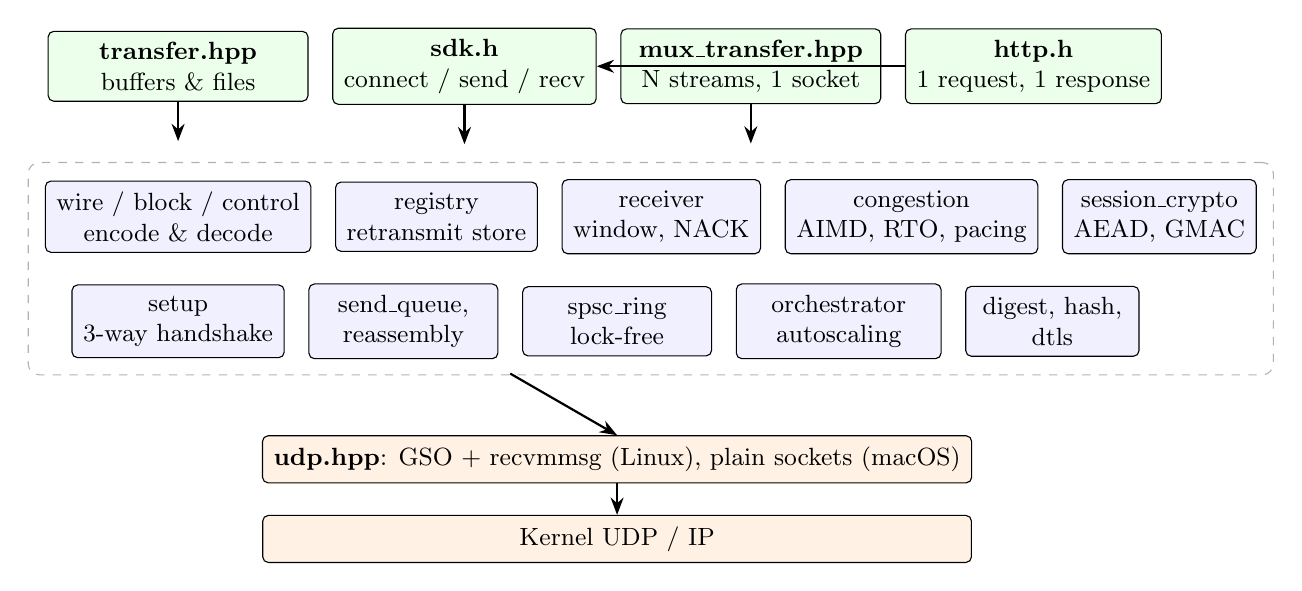
\begin{tikzpicture}[node distance=4mm and 3mm, every node/.style={font=\small}]
  \node[api,minimum width=3.3cm] (t) {\textbf{transfer.hpp}\\buffers \& files};
  \node[api,minimum width=3.3cm,right=of t] (s) {\textbf{sdk.h}\\connect / send / recv};
  \node[api,minimum width=3.3cm,right=of s] (m) {\textbf{mux\_transfer.hpp}\\N streams, 1 socket};
  \node[api,minimum width=3.0cm,right=of m] (h) {\textbf{http.h}\\1 request, 1 response};
  \node[core,below=10mm of t,minimum width=2.6cm] (w) {wire / block / control\\encode \& decode};
  \node[core,right=of w,minimum width=2.4cm] (r) {registry\\retransmit store};
  \node[core,right=of r,minimum width=2.4cm] (rx) {receiver\\window, NACK};
  \node[core,right=of rx,minimum width=2.6cm] (cc) {congestion\\AIMD, RTO, pacing};
  \node[core,right=of cc,minimum width=2.2cm] (cr) {session\_crypto\\AEAD, GMAC};
  \node[core,below=4mm of w,minimum width=2.6cm] (su) {setup\\3-way handshake};
  \node[core,right=of su,minimum width=2.4cm] (q) {send\_queue,\\reassembly};
  \node[core,right=of q,minimum width=2.4cm] (ring) {spsc\_ring\\lock-free};
  \node[core,right=of ring,minimum width=2.6cm] (o) {orchestrator\\autoscaling};
  \node[core,right=of o,minimum width=2.2cm] (d) {digest, hash,\\dtls};
  \node[io,below=10mm of ring,minimum width=9cm] (u) {\textbf{udp.hpp}: GSO + \code{recvmmsg} (Linux), plain sockets (macOS)};
  \node[io,below=4mm of u,minimum width=9cm] (k) {Kernel UDP / IP};
  \begin{scope}[on background layer]
    \node[draw=black!30,dashed,rounded corners,fit=(w)(cr)(su)(d),inner sep=6pt] {};
  \end{scope}
  \draw[arr] (h) -- (s);
  \draw[arr] ($(t.south)+(0,0)$) -- ++(0,-5mm);
  \draw[arr] ($(s.south)+(0,0)$) -- ++(0,-5mm);
  \draw[arr] ($(m.south)+(0,0)$) -- ++(0,-5mm);
  \draw[arr] (u) -- (k);
  \draw[arr] ($(q.south)!0.5!(ring.south)+(0,-2mm)$) -- (u.north);
\end{tikzpicture}}
\caption{Layered structure of the repository: public APIs (green), protocol core (blue), platform I/O (orange).}\label{fig:layers}
\end{figure}

The public APIs are:
\begin{itemize}
  \item \code{transfer.hpp}: \code{send_buffer}, \code{receive_buffer}, \code{send_file} and \code{receive_file};
  \item \code{sdk.h}: a C API with \code{fuse_listen}, \code{fuse_accept}, \code{fuse_connect},
    \code{fuse_send}, \code{fuse_recv} and \code{fuse_close};
  \item \code{mux_transfer.hpp}: \code{send_multiplexed} and \code{receive_multiplexed};
  \item \code{http.h}: one HTTP/1.1 request and one response over an SDK connection.
\end{itemize}

They build into the libraries listed in Table~\ref{tab:targets}.

\begin{table}[H]
\centering\small
\caption{CMake library targets.}\label{tab:targets}
\begin{tabularx}{\linewidth}{lXl}
\toprule
\textbf{Target} & \textbf{Contents} & \textbf{Installed} \\
\midrule
\code{fuse::proto} & Protocol core: block, control, registry, receiver, UDP, SETUP, reassembly, DTLS, orchestrator, session crypto, digest & yes \\
\code{fuse::sdk} & The three transports (\code{transfer.cpp}, \code{mux_transfer.cpp}, \code{sdk.cpp}), linking \code{fuse::proto} & no$^{*}$ \\
\code{fuse::http} & HTTP mapping (\code{http.cpp}) & no$^{*}$ \\
\code{fuse::fuse} & Legacy C scaffold (QUIC-like long header, variable-length integers); unused by the protocol & yes \\
\bottomrule
\multicolumn{3}{l}{\footnotesize $^{*}$Released from the separate \code{fuse-sdk} repository.}
\end{tabularx}
\end{table}

Two build options matter most:
\begin{itemize}
  \item \code{FUSE_WITH_CRYPTO} (on by default) links wolfSSL~\cite{wolfssl}. The build can fetch wolfSSL and
    compiles it with AES-NI assembly: wolfSSL's own CMake build had silently used software AES, at 151~MB/s
    against 4,852~MB/s with the assembly enabled.
  \item Without crypto, every cryptographic entry point fails closed, and a request for encryption returns
    \code{Unsupported}.
\end{itemize}

\section{The three transports at a glance}

\begin{table}[H]
\centering\small
\caption{The three transports.}\label{tab:transports}
\begin{tabularx}{\linewidth}{>{\raggedright\arraybackslash}p{2.4cm}>{\raggedright\arraybackslash}X>{\raggedright\arraybackslash}X>{\raggedright\arraybackslash}X}
\toprule
 & \textbf{Bulk transfer} & \textbf{SDK} & \textbf{Multiplexed} \\
\midrule
Unit & one buffer or file, split into \emph{lanes} & messages on a connection & one buffer over $N$ streams \\
Ports & one per lane (\code{base_port}$+i$) & one listen port, then a fresh port per connection & one \\
Threads & sender: one per lane; receiver: one reader per lane, $K$ writers, one retransmission consumer & one pump thread per connection & autoscaling pool \\
Session setup & per-lane StreamStart with Retry token\vviii & HELLO / HELLO-ACK & SETUP, then per-stream StreamStart \\
Encryption & AES-256-GCM per block; GMAC on control\vviii; key epochs\vviii & AES-256-GCM on DATA only & none \\
v8 hardening & complete & deferred & SACK, RTO, slow start, validation \\
\bottomrule
\end{tabularx}
\end{table}

\section{Evolution of the wire protocol}

The first byte of every datagram is the protocol version. Each increment was an on-wire change, and the
comment above the constant in \code{wire.hpp} records why (Table~\ref{tab:versions}).

\begin{table}[H]
\centering\small
\caption{Protocol versions and the reason for each change.}\label{tab:versions}
\begin{tabularx}{\linewidth}{c>{\raggedright\arraybackslash}p{5cm}X}
\toprule
\textbf{v} & \textbf{Change} & \textbf{Reason} \\
\midrule
1 & Block header, registry, bitmask, ACK/NACK & Stage 1 reliability core \\
2 & Explicit byte offset in DATA & Block size adapts mid-stream, so $\mathit{seq}\times\mathit{size}$ misplaces data \\
3 & Multi-word bitmask; handshake nonce & Windows over 64 blocks; a stale ACK must not confirm a new session \\
4 & Server salt in HELLO-ACK & Retried HELLOs could derive identical keys with both sequence numbers at 0, an AES-GCM nonce collision \\
5 & Two-byte window size & Raise the window from 255 to 1,024 blocks; the old field capped throughput on any real bandwidth-delay product \\
6 & Base offset and total size in StreamStart & Write each block directly to its final file position \\
7 & File id, ResumeRanges, FileDigest & Resumable file reception with whole-file verification \\
8 & Control-plane authentication, AAD fix, key epochs, Retry, path validation, SETUP nonce, receive window, extensions, version-mismatch reply & The security and correctness review (Chapter~\ref{ch:security}) \\
\bottomrule
\end{tabularx}
\end{table}

\section{Design principles of the implementation}\label{sec:principles}

The code base is small, but it follows a consistent set of principles. They explain many choices that look
unusual in isolation.

\paragraph{Staged construction with acceptance tests.} The protocol was built in stages, each with its own
acceptance test:

\smallskip
\begin{center}\small
\begin{tabular}{@{}ll@{\qquad}ll@{}}
\toprule
\textbf{Stage} & \textbf{Scope} & \textbf{Stage} & \textbf{Scope} \\
\midrule
0 & framing & 4 & per-stream flags \\
1 & blocks and the received bitmask & 5 & congestion control \\
1.5 & control messages & 6 & CPU pinning \\
2 & SETUP & 7 & encryption \\
3 & worker threads & 8 & benchmarks \\
\bottomrule
\end{tabular}
\end{center}
\smallskip

\noindent When a measurement contradicted a stage, the stage was removed rather than kept because it had been
planned. CPU pinning made transfers about 6\% slower, so Stage~6 was deleted, and the reason is recorded in
\code{orchestrator.hpp}.

\paragraph{Pure state machines; the caller owns I/O and time.} The SETUP handshake, the receiver window, the
sender registry and the congestion controller never touch a socket or read a clock. They receive the current
time as an argument and write any datagram they want to send into a buffer supplied by the caller. As a result:
\begin{itemize}
  \item tests can drive them with a virtual clock and injected loss, so ``retransmits after 50~ms'' is a
    deterministic unit test rather than a sleep;
  \item the same logic serves three transports with different threading models.
\end{itemize}
Loops that depend on time are bounded: the congestion controller processes at most 4,096 epochs per call, so a
clock jump cannot make it spin.

\paragraph{A single place for byte order.} Only the \code{put_u8}\ldots\code{put_u64} and
\code{get_u8}\ldots\code{get_u64} helpers in \code{wire.hpp} touch raw wire bytes. They are all big-endian, and
each returns the number of bytes it consumed, so cursor arithmetic looks the same everywhere. Every message has
an encoder that returns the encoded length (zero if it does not fit) and a decoder that returns false on a
version mismatch, the wrong type or truncation. A malformed datagram is therefore dropped at one obvious place.

\paragraph{Fixed-size storage and no allocation on the hot path.}
\begin{itemize}
  \item A registry slot embeds its whole payload array rather than a pointer.
  \item The receiver's bitmask and gap timers are fixed arrays sized by the maximum window.
  \item Messages are plain structures with fixed arrays.
\end{itemize}
A test that replaces the global \code{operator new} proves that the Stage~1 send and receive loop allocates
nothing after setup. This avoids allocator latency and jitter, and a hostile length field cannot grow a fixed
array. The cost is memory sized for the worst case, which is visible in the SDK (Section~\ref{sec:sdk}).

\paragraph{Every wire field is hostile.} Lengths, offsets and counts from the network are bounded before any
arithmetic is done with them, and in an order that cannot overflow. For example, a block's placement is checked
as $\mathit{offset}\le\mathit{total} \wedge \mathit{len}\le\mathit{total}-\mathit{offset}$, never as
$\mathit{offset}+\mathit{len}\le\mathit{total}$, because an offset close to $2^{64}$ would wrap the sum. A claimed
transfer size that cannot be allocated fails the transfer with \code{ResourceLimit} instead of throwing out of a
thread.

\paragraph{Fail closed.}
\begin{itemize}
  \item With no cryptographic backend, encryption requests are refused rather than downgraded.
  \item With no secure random source, the process aborts rather than use a predictable nonce.
  \item If sealing a block fails, the batch stops rather than emit plaintext.
  \item A cipher object refuses to be keyed twice, because re-keying is how a (key, nonce) pair could repeat.
  \item Since version~8, under a pre-shared key, nothing unsigned is acted upon.
\end{itemize}

\paragraph{Ownership through RAII.}
\begin{itemize}
  \item Sockets are move-only objects, and ciphers are uniquely owned.
  \item The digest thread of a sending lane is joined on every exit path by a small guard object.
  \item The SDK counts the application threads inside \code{fuse_send} and \code{fuse_recv} with an RAII guard,
    so that closing a connection can wait for them.
  \item Key material is wiped after use.
\end{itemize}
Lane functions have a dozen early exits (cancellation, timeout, abort, authentication failure), and RAII is what
keeps the cleanup correct on all of them.

\paragraph{A concurrency model chosen per component.} Three patterns are used, each where it fits:
\begin{enumerate}
  \item \emph{Thread confinement}. A bulk-transfer lane owns its socket, registry, receiver state and ciphers
    outright, so nothing on its per-packet path is locked.
  \item \emph{Lock-free single-producer, single-consumer rings} between a lane's socket reader and the writer
    threads.
  \item \emph{One mutex per stream or connection} in the multiplexed transfer and the SDK, where several
    threads touch the same stream.
\end{enumerate}
Shared counters use the weakest correct memory ordering: relaxed for progress statistics, release and acquire
for the flags that publish state.

\paragraph{Hiding dependencies.}
\begin{itemize}
  \item wolfSSL types appear in no public header; a cipher holds its context as an opaque pointer.
  \item Platform differences are confined to three files: \code{udp_linux.cpp} (segmentation offload,
    \code{recvmmsg}, MTU query), \code{udp_darwin.cpp} (one system call per datagram) and
    \code{udp_common.cpp}.
\end{itemize}

\paragraph{Time, not counts.}
\begin{itemize}
  \item All timing uses a monotonic nanosecond clock, and differences are taken modulo $2^{64}$.
  \item Retries are bounded by elapsed time. The original StreamStart handshake gave up after
    $200\times200~\mu$s $=40$~ms, so it failed on any path with a longer round trip. It now retries with
    exponential backoff until a connect timeout.
  \item The sender keeps two progress clocks. One paces retransmission. The other, which only moves when an
    acknowledgement confirms new data, enforces the user's timeout. A local send to a dead peer keeps
    ``succeeding'', so using the first clock for the timeout made the loop unbounded.
\end{itemize}

\paragraph{A C ABI where stability matters.} The SDK is plain C. It uses opaque handles, a status enumeration,
and a configuration structure initialised by a function, so that fields can be added without breaking callers.
It is the stable interface for bindings to other languages.

\paragraph{Comments state the invariant and its history.} Comments explain \emph{why}, often naming the bug
that motivated a line and the roadmap number of its fix. Protocol code is mostly invariants, and a future change
that breaks one should run into the comment that states it.

\chapter{Wire Format}\label{ch:wire}

This chapter specifies the datagrams Fuse exchanges. The normative description is \code{docs/PROTOCOL.md} in
the repository~\cite{repo}; here we explain the purpose of each field and the code that reads it. All
multi-byte integers are big-endian and all sizes are in bytes.

\section{Outer header and message types}

Every datagram begins with a two-byte outer header, \code{[version:1][msg_type:1]}. A receiver rejects any
datagram whose version it does not understand before it interprets a single further byte. A receive loop
dispatches on the message type by peeking at the header alone. Table~\ref{tab:msgtypes} lists the message types.

\begin{table}[H]
\centering\small
\caption{Message types (\texttt{wire.hpp}). Sizes exclude the 24-byte authentication trailer (Section~\ref{sec:wirecrypto}).}\label{tab:msgtypes}
\begin{tabular}{rllll}
\toprule
\textbf{Type} & \textbf{Name} & \textbf{Direction} & \textbf{Used by} & \textbf{Size} \\
\midrule
0 & DATA & sender $\to$ receiver & all & $31+\text{payload}$ \\
1 & HEARTBEAT & either & none (defined only) & 12 \\
2 & ACK & receiver $\to$ sender & all & 160 \\
3 & NACK & receiver $\to$ sender & all & $6+8n$ \\
4 & SETUP\_DATA & initiator $\to$ responder & mux & $7+9s+2+\text{ext}$ \\
5 & SETUP\_HASH\_REPLY & responder $\to$ initiator & mux & 18 \\
6 & SETUP\_FINACK & initiator $\to$ responder & mux & 18 \\
7 & STREAM\_START & sender $\to$ receiver & transfer, mux & $80+\text{ext}$ \\
8 & HELLO & client $\to$ server & SDK & 26 \\
9 & HELLO\_ACK & server $\to$ client & SDK & 42 \\
10 & CLOSE & either & SDK & 2 \\
11 & STREAM\_CLOSE & either & transfer & 13 \\
12 & RESUME\_RANGES & receiver $\to$ sender & transfer & $19+16n$ \\
13 & FILE\_DIGEST & both (echoed) & transfer & 44 \\
14 & RETRY\vviii & receiver $\to$ sender & transfer & 20 \\
15 & PATH\_CHALLENGE\vviii & either & transfer & 20 \\
16 & PATH\_RESPONSE\vviii & either & transfer & 20 \\
\bottomrule
\end{tabular}
\end{table}

\subsection{Version mismatch\vviii}

Before version~8, a datagram carrying an unknown version was met with silence, and the peer's user eventually
saw only a timeout. A receiver now answers such a datagram, at most once per 100~ms, with a three-byte reply
\code{[our_version][0xFF][our_version]}. This layout is fixed permanently, independently of the protocol
version, so any future version can recognise it.
\begin{itemize}
  \item The reply is never larger than the datagram that triggered it, so it cannot be used to amplify an attack.
  \item A mismatch reply is itself never answered; otherwise two mismatched peers would exchange replies forever.
  \item The bulk-transfer and multiplexed senders report the condition as \code{VersionMismatch}.
\end{itemize}

\subsection{Extensions\vviii}

STREAM\_START and SETUP\_DATA end in an extension area,
\code{[ext_len:2]} followed by entries \code{[type:2][len:2][value]}, at most 256 bytes in total. The
rules are:
\begin{itemize}
  \item a receiver ignores extension types it does not know;
  \item it refuses the whole message if it finds an unknown \emph{critical} type (top bit set,
    $\mathit{type}\ge\text{0x8000}$);
  \item version~8 defines no types, so every critical type is refused today.
\end{itemize}
Before this mechanism, any new field required a version change, and a version change breaks interoperability
outright. A type-length-value area with a critical bit is the established remedy, used by IPv6 options, TLS
extensions and QUIC transport parameters~\cite{rfc9000}.

\section{Data plane}

\subsection{DATA}

\begin{lstlisting}
[version:1][type=0:1]
[stream_id:2][seq_no:8][flags:1][payload_len:2][offset:8]      21-byte block header
[send_time_ns:8]                                               echoed for RTT measurement
[payload: payload_len bytes]                                   ciphertext + 16-byte tag under a PSK
\end{lstlisting}

The fields are:
\begin{itemize}
  \item \code{stream_id} identifies the lane, stream or direction.
  \item \code{seq_no} is per stream, starts at zero and is never reused; a retransmission keeps its original
    number.
  \item \code{flags} has two bits: 0x01 marks a retransmission, 0x02 marks the last block of a stream.
  \item \code{payload_len} is at most 16,384 and includes the authentication tag when encrypted.
  \item \code{offset} is the block's byte position within its stream. It has been carried explicitly since
    version~2 because the block size changes during a transfer, so it cannot be derived from the sequence
    number.
\end{itemize}

The 31-byte prefix plus the default 1,200-byte payload, the 28 bytes of IPv4 and UDP headers and a 16-byte tag
come to 1,275 bytes, safely below a 1,500-byte MTU.

\code{send_time_ns} is the sender's clock \emph{plus a random per-stream offset}\vviii. Only the sender ever
interprets the value; the receiver merely echoes it. Placing the raw monotonic clock on the wire would reveal
the host's uptime to any observer. The round-trip time is computed as a wrap-safe difference in the same offset
domain, and an echo from the future or older than one minute is discarded.

\subsection{ACK}

\begin{lstlisting}
[outer][stream_id:2][base_seq_no:8][received_bitmask:16 x 8][echoed_send_time:8][nonce:8][rwnd:4]
\end{lstlisting}

\begin{itemize}
  \item \code{base_seq_no} is cumulative: every block below it has been received and written.
  \item Bit $i$ of the 1,024-bit \code{received_bitmask} reports block $\mathit{base}+i$. This is the selective
    part of the acknowledgement.
  \item \code{echoed_send_time} is the send time of the highest-numbered block accepted so far.
  \item \code{nonce} echoes the StreamStart nonce, so that a stale acknowledgement from an earlier session on
    the same port cannot confirm a new one.
  \item \code{rwnd}\vviii{} is the number of further unacknowledged blocks the receiver can currently hold;
    0xFFFFFFFF means unlimited.
\end{itemize}

\subsection{NACK and HEARTBEAT}

A NACK, \code{[outer][stream_id:2][count:2][missing_seq_no:8]}$\times$\code{count}, names up to 1,024
missing sequence numbers. Its length is bounded by the window, because nothing outside the window can be
tracked, so a full-window NACK (8,198 bytes) is the largest control datagram and receive buffers are sized for
it. A HEARTBEAT, \code{[outer][stream_id:2][highest_seq_no:8]}, is defined but never sent today, so idle SDK
connections have no liveness signal (Chapter~\ref{ch:conclusion}).

\section{Bulk-transfer control messages}

\begin{table}[H]
\centering\small
\caption{STREAM\_START (80 bytes plus extensions).}\label{tab:streamstart}
\begin{tabularx}{\linewidth}{lcX}
\toprule
\textbf{Field} & \textbf{Size} & \textbf{Meaning} \\
\midrule
\code{stream_id} & 2 & lane index \\
\code{total_blocks} & 8 & always 0 from the transfer API (the block size adapts) \\
\code{block_size} & 2 & initial block size \\
\code{total_bytes} & 8 & length of this lane's shard \\
\code{session_salt} & 16 & HKDF salt; all zero means unencrypted \\
\code{nonce} & 8 & random per lane and attempt; echoed in every reply \\
\code{stream_base_offset} & 8 & where the shard sits in the whole file \\
\code{file_total_bytes} & 8 & size of the whole transfer \\
\code{file_id} & 8 & identity of the file, for resume; 0 means not resumable \\
\code{token} & 8 & address-validation token from the receiver's RETRY; 0 on the first attempt\vviii \\
\code{ext_len} + ext & $2+n$ & extension area\vviii \\
\bottomrule
\end{tabularx}
\end{table}

\begin{description}[style=nextline,leftmargin=1.2cm]
  \item[RETRY (20 bytes)\vviii] \code{[stream_id:2][nonce:8][token:8]}. It is deliberately smaller than the
    StreamStart it answers, so a spoofed source address gains no amplification.
  \item[PATH\_CHALLENGE, PATH\_RESPONSE (20 bytes each)\vviii] \code{[stream_id:2][nonce:8][challenge:8]}; the
    response echoes the challenge.
  \item[RESUME\_RANGES ($19+16n$ bytes)] \code{[stream_id:2][nonce:8][flags:1][part:2][parts:2][count:2]}
    followed by \code{count} pairs \code{(offset:8, length:8)}. The pairs are the parts of the lane the
    receiver still needs, relative to the stream. A long list is split across datagrams of at most 64 ranges
    each, about 1~KB. Flag 0x01 means the transfer is resuming. A fresh transfer answers with one range covering
    the whole lane.
  \item[STREAM\_CLOSE (13 bytes)] \code{[stream_id:2][nonce:8][reason:1]}. The reason is 0 for finished, 1 for
    aborted, or 2 for authentication failed\vviii. The message is sent three times and never acknowledged.
  \item[FILE\_DIGEST (44 bytes)] \code{[stream_id:2][nonce:8][digest:32]}. It is sent on lane~0 at the end of a
    resumed transfer, and the receiver's echo serves as the acknowledgement.
\end{description}

\section{SDK and SETUP messages}

\begin{itemize}
  \item \textbf{HELLO} (26 bytes, \code{salt_c:16, challenge:8}) arrives on the server's listen port.
  \item \textbf{HELLO\_ACK} (42 bytes, \code{salt_s:16, proof:24}) is sent from a fresh per-connection socket.
    Under a pre-shared key, the proof is the client's challenge sealed with the new session key, which shows the
    server holds the key. The client adopts the source address of the HELLO\_ACK as its peer. This is how a
    single listen port serves many connections without connection identifiers, as in TFTP~\cite{rfc1350}.
  \item \textbf{CLOSE} (2 bytes) is a graceful teardown.
\end{itemize}

SETUP\_DATA carries:
\begin{itemize}
  \item \code{[protocol_version:1][num_workers:2][num_streams:2]};
  \item then, for each of at most 64 streams, \code{[stream_id:2][worker_id:2][flags:1][block_size:2][window_size:2]};
  \item then the extension area\vviii.
\end{itemize}
The stream flags are 0x01 \code{LOSSLESS}, 0x02 \code{ORDERED} and 0x04 \code{COALESCE}. SETUP\_HASH\_REPLY and
SETUP\_FINACK both carry \code{[hash:8][responder_nonce:8]}. The hash is FNV-1a-64~\cite{fnv} of the SETUP body
exactly as the responder received it. The responder nonce\vviii{} is drawn fresh for each configuration offered,
and the FINACK must echo it.

\section{Encryption on the wire}\label{sec:wirecrypto}

Table~\ref{tab:crypto} summarises the cryptographic constructions of the bulk-transfer path.

\begin{table}[H]
\centering\small
\caption{Cryptographic constructions (\texttt{session\_crypto.cpp}, \texttt{transfer.cpp}).}\label{tab:crypto}
\begin{tabularx}{\linewidth}{>{\raggedright\arraybackslash}p{2.7cm}X}
\toprule
\textbf{Item} & \textbf{Construction} \\
\midrule
Session key & HKDF-SHA256~\cite{rfc5869}: Extract(salt, PSK), then Expand-Label(\code{"fuse2 "}, \code{"session key"}, empty context, 32 bytes). The salt is the StreamStart salt (transfer) or $\mathit{salt}_c\,\|\,\mathit{salt}_s$ (SDK). \\
Data key\vviii & Expand-Label(session key, \code{"lane key"}, $\mathit{lane}{:}2\,\|\,(\mathit{seq}\gg22){:}8$) \\
Control key\vviii & Expand-Label(session key, \code{"control key"}, empty) \\
DATA AEAD & AES-256-GCM~\cite{nist-gcm}. Nonce $=\mathit{lane}{:}2\,\|\,\mathit{seq}{:}8\,\|\,\text{0x0000}$. AAD $=\mathit{lane}\,\|\,\mathit{seq}\,\|\,\mathit{offset}\,\|\,\mathit{flags}$, with the retransmission bit cleared\vviii. The 16-byte tag follows the ciphertext. \\
Control trailer\vviii & $\mathit{ctr}{:}8\,\|\,\mathit{tag}{:}16$ appended to every control datagram except RETRY, the version-mismatch reply and STREAM\_CLOSE(reason~2). The tag is a GMAC (GCM with empty plaintext) over the whole datagram including \code{ctr}. Nonce $=\mathit{lane}{:}2\,\|\,\mathit{ctr}{:}8\,\|\,\mathit{dir}{:}1\,\|\,\text{0x01}$, where $\mathit{dir}$ is 0 for the data sender and 1 for the data receiver. \\
\bottomrule
\end{tabularx}
\end{table}

\noindent Three properties keep the nonce spaces disjoint:
\begin{itemize}
  \item data nonces end in 0x0000 and control nonces in 0x01, so the two spaces cannot meet even before the keys
    differ;
  \item the direction byte separates the two endpoints, which share the key and the lane;
  \item a pair $(\mathit{lane},\mathit{seq})$ never repeats within a session, and the session key is fresh for
    every salt.
\end{itemize}

\section{Constants}

\begin{table}[H]
\centering\small
\caption{Constants worth remembering.}\label{tab:constants}
\begin{tabular}{llr>{\raggedright\arraybackslash}p{5.6cm}}
\toprule
\textbf{Constant} & \textbf{Defined in} & \textbf{Value} & \textbf{Meaning} \\
\midrule
\code{kProtocolVersion} & \code{wire.hpp} & 8 & first byte of every datagram \\
\code{kDefaultPayloadSize} & \code{wire.hpp} & 1,200 & safe under a 1,500-byte MTU \\
\code{kMaxPayloadSize} & \code{wire.hpp} & 16,384 & block growth ceiling \\
\code{kMaxWindow} & \code{wire.hpp} & 1,024 & blocks in flight per stream \\
\code{kDataPrefixSize} & \code{wire.hpp} & 31 & DATA bytes before the payload \\
\code{kMaxExtensionBytes} & \code{wire.hpp} & 256 & extension area limit \\
\code{kMaxStreams} & \code{setup.hpp} & 64 & streams per SETUP \\
\code{kDefaultSetupTimeoutNs} & \code{setup.hpp} & 50 ms & SETUP retransmission interval \\
\code{kControlTrailerLen} & \code{session_crypto.hpp} & 24 & counter plus GMAC tag \\
\code{kKeyEpochShift} & \code{session_crypto.hpp} & 22 & $2^{22}$ blocks per data key \\
\code{kMinPreSharedKeyLen} & \code{transfer.cpp} & 16 & shorter keys are refused \\
\bottomrule
\end{tabular}
\end{table}

\chapter{Building Blocks of the Protocol Core}\label{ch:components}

Each component below is a small class or set of functions in \code{include/fuse/proto/}, with its own test file
in \code{tests/proto/}. None of them owns a thread or reads a clock.

\section{UDP socket with batched I/O}\label{sec:udp}

\code{UdpSocket} (\code{udp.hpp}) is a move-only wrapper around one bound UDP socket. Its receive buffers are
large enough for the biggest datagram, so the kernel never truncates a block. Peer addresses are carried in an
opaque, comparable \code{PeerAddr} that may hold an IPv4 or an IPv6 address.

Its two batched operations carry the data path:

\begin{description}[style=nextline,leftmargin=1.2cm]
  \item[\code{send_segmented}] passes the kernel one buffer of back-to-back datagrams in a single
    \code{sendmsg}, tagged with the \code{UDP_SEGMENT} control message (generic segmentation offload,
    Linux~4.18)~\cite{gso}. The kernel or the network card cuts it into ordinary datagrams, so the wire sees
    normal MTU-sized packets.
    \begin{itemize}
      \item If the kernel refuses the call (EIO, ENOTSUP or EINVAL), a flag latches and the caller falls back to
        one \code{sendto} per datagram.
      \item The bulk transfer caps a batch at 64 segments. With a small block size a batch could otherwise
        exceed the kernel's per-call segment limit, and the resulting EINVAL cannot be told apart from ``this
        route has no offload'', so offload would be disabled for the rest of the transfer.
    \end{itemize}
  \item[\code{recv_batch}] receives up to $N$ datagrams in one \code{recvmmsg}~\cite{recvmmsg} with
    \code{MSG_WAITFORONE}, and records the source address of \emph{every} datagram.
    \begin{itemize}
      \item Without \code{MSG_WAITFORONE}, the call would block until all $N$ datagrams had arrived.
      \item The per-datagram source address is what allows path validation to notice a NAT rebinding in the
        middle of a batch.
    \end{itemize}
\end{description}

One system call per datagram limits a modern host to about 213,000 datagrams per second whatever the link
speed; batching amortises that cost.

\code{path_mtu}\vviii{} connects a temporary socket to the destination and reads the kernel's route MTU
(\code{IP_MTU} or \code{IPV6_MTU}). Together with the IP and UDP header overhead (28 bytes for IPv4, 48 for IPv6)
it bounds how far the block size may grow. On macOS the MTU cannot be queried this way, so blocks do not grow
there. Version~8 also opens each sending socket in the destination's address family; earlier versions always
opened IPv4 sockets, which made IPv6 hosts unreachable.

\section{Sender registry and selective acknowledgement}\label{sec:registry}

The \code{SenderRegistry} is the store from which lost blocks are resent. It is a circular array of
$W$ slots (the stream's window size) indexed by $\mathit{seq}\bmod W$. Each slot holds:
\begin{itemize}
  \item the sequence number, send time, byte offset and length;
  \item the block's original flags and a validity bit;
  \item the payload itself, embedded in a 16~KiB array.
\end{itemize}

The registry has three operations:
\begin{itemize}
  \item \code{store} overwrites the slot a sequence number maps to.
  \item \code{lookup} returns the slot only if it is valid \emph{and} still holds exactly that sequence number.
    Otherwise the requested block has already been confirmed or overwritten.
  \item \code{confirm} releases a slot once an acknowledgement covers it.
\end{itemize}
The flags are stored because a retransmission must add the retransmission bit without losing the last-block
bit: a retransmitted last block is still the last block, and the receiver has no other way to learn that the
stream has ended.

\paragraph{Applying an acknowledgement\vviii.} Every sender digests acknowledgements through one function,
\code{apply_ack} (\code{registry.cpp:52}), which works in three steps:
\begin{enumerate}
  \item \emph{Cumulative part.} If the acknowledgement's base exceeds the sender's base, every slot up to
    $\min(\mathit{ack.base}, \mathit{next\_seq})$ is confirmed. The clamp matters: an unauthenticated
    acknowledgement must not confirm blocks that were never sent.
  \item \emph{Selective part.} Every set bit $i$ of the bitmask, enumerated with a count-trailing-zeros
    instruction, confirms block $\mathit{ack.base}+i$ if it is below \code{next_seq}.
  \item \emph{Result.} The function returns the number of payload bytes newly confirmed, and raises
    \code{received_end} to one past the highest block the acknowledgement shows as received.
\end{enumerate}

Before version~8 the bitmask was ignored, so burst losses were repaired by NACKs alone and blocks the receiver
already held were resent. The \code{received_end} value lets the retransmission timer distinguish blocks that
are lost (unacknowledged, below it) from blocks that may still be in flight (above it). This is the same
distinction SACK-based recovery makes in TCP~\cite{rfc2018} and QUIC~\cite{rfc9002}.

\section{Receiver window and loss detection}\label{sec:receiver}

\code{ReceiverStream} tracks one incoming stream. Its state is:
\begin{itemize}
  \item a base sequence number, below which everything has been delivered;
  \item a bitmask of received blocks;
  \item the highest sequence number seen, and the send time to echo;
  \item two timers per window position: when the gap at that position was first seen, and when it was last
    reported.
\end{itemize}
In version~8 the bitmask and the timers are \emph{rings} indexed by $\mathit{seq}\bmod 1024$
(Figure~\ref{fig:ring}). Earlier versions shifted whole arrays every time the base moved, which made each
receive $O(W)$.

\begin{figure}[H]
\centering
\fitwidth{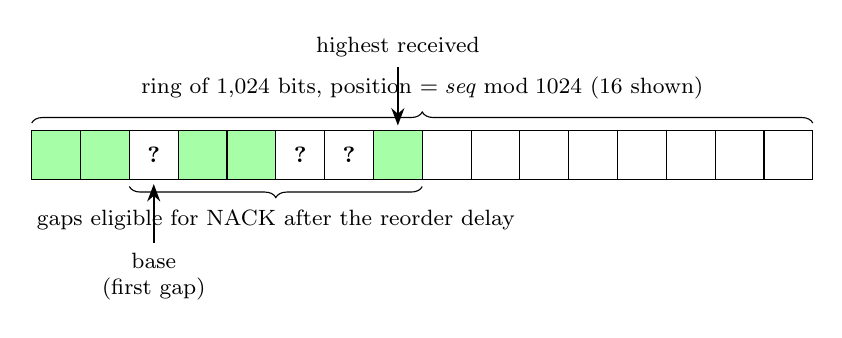
\begin{tikzpicture}[x=6.2mm,y=6.2mm,font=\footnotesize]
  \foreach \i/\c in {0/green!35,1/green!35,2/white,3/green!35,4/green!35,5/white,6/white,7/green!35,8/white,9/white,10/white,11/white,12/white,13/white,14/white,15/white}{
    \draw[fill=\c] (\i,0) rectangle ++(1,1);
  }
  \node at (2.5,0.5) {\textbf{?}}; \node at (5.5,0.5) {\textbf{?}}; \node at (6.5,0.5) {\textbf{?}};
  \draw[arr] (2.5,-1.3) node[below,lbl]{base\\(first gap)} -- (2.5,-0.1);
  \draw[arr] (7.5,2.3) node[above,lbl]{highest received} -- (7.5,1.1);
  \draw[decorate,decoration={brace,amplitude=4pt,mirror}] (2,-0.15) -- (8,-0.15) node[midway,below=5pt,lbl]{gaps eligible for NACK after the reorder delay};
  \draw[decorate,decoration={brace,amplitude=4pt}] (0,1.15) -- (16,1.15) node[midway,above=5pt,lbl] {ring of 1,024 bits, position $=\mathit{seq}\bmod 1024$ (16 shown)};
\end{tikzpicture}}
\caption{The receive window. Green positions have arrived. The base sits on the first gap; positions between
the base and the highest block received are candidate losses.}\label{fig:ring}
\end{figure}

\paragraph{Receiving a block.} \code{on_receive} (\code{receiver.cpp:135}) handles one arriving sequence
number:
\begin{enumerate}
  \item Below the base, it returns \emph{Duplicate}.
  \item A full window or more beyond the base, it returns \emph{OutOfWindow} and counts the overflow.
  \item Already marked received, it returns \emph{Duplicate}.
  \item Otherwise it marks the block received. If the block is a new highest, every position between the
    previous highest and this block has just become a gap, and each gets its first-missing timestamp, exactly
    once.
  \item Finally it slides the base over the contiguous received prefix, clearing each bit and both timers
    exactly once as it passes. This keeps the invariant that positions below the base are always clear, which
    is what makes the ring unambiguous.
\end{enumerate}
Each position is touched a constant number of times over its life, so receiving is $O(1)$ amortised. The
relative bitmask an acknowledgement needs, in which bit $i$ means $\mathit{base}+i$, is assembled from the ring
word by word with two shifts per word.

\paragraph{Reporting losses.} \code{collect_nacks} walks the clear bits between the base and the highest block
received, a word at a time. It reports a gap only if two conditions hold:
\begin{itemize}
  \item the gap has lasted longer than a \emph{reorder delay};
  \item the gap was not reported within a \emph{re-NACK interval}.
\end{itemize}
A stream that is not \code{LOSSLESS} never reports losses. The two conditions exist because a block that is
merely late must not be treated as lost, and re-reporting a gap before its retransmission could possibly arrive
only causes duplicate retransmissions. The bulk-transfer receiver scales both intervals with its own estimate of
the round-trip time (Section~\ref{sec:recovery}).

\section{Congestion control}\label{sec:cc}

Each \code{LOSSLESS} stream has its own \code{CongestionController} (\code{congestion.hpp}). Keeping congestion
state per stream rather than per connection is the deliberate difference from QUIC on which the design rests.
The controller's window is in abstract units: the bulk transfer interprets them as units of the configured
block size\vviii, and the multiplexed transfer as blocks.

\paragraph{RTT estimation.} The controller follows RFC~6298~\cite{rfc6298}. The first sample $R$ sets
$\mathit{SRTT}=R$ and $\mathit{RTTVAR}=R/2$. Each later sample updates
\[
\mathit{RTTVAR}\leftarrow\tfrac34\mathit{RTTVAR}+\tfrac14\lvert \mathit{SRTT}-R\rvert,\qquad
\mathit{SRTT}\leftarrow\tfrac78\mathit{SRTT}+\tfrac18R .
\]

\paragraph{AIMD epochs and slow start.} The controller makes one decision per elapsed SRTT
(Figure~\ref{fig:ccfsm}):
\begin{itemize}
  \item If a loss (a NACK, or the first timeout of a run) was observed during the epoch, the window halves, but
    not below a floor of two, and slow start ends.
  \item In slow start\vviii, a clean epoch doubles the window up to the cap.
  \item In congestion avoidance, a run of clean epochs adds a fixed step. Both transports grow by 16 units after
    one clean epoch.
\end{itemize}
Slow start was added because, without it, the window had to climb from one eighth of the cap a few units per
round trip, which takes many round trips on a long path. It is opt-in, so existing users of the component keep
their behaviour unchanged.

\begin{figure}[H]
\centering
\fitwidth{\begin{tikzpicture}[node distance=2.2cm and 4.2cm, >={Stealth[length=2.2mm]}, every edge/.style={draw,thick}]
  \node[st,minimum width=2.6cm] (ss) {Slow start};
  \node[st,minimum width=2.6cm,right=of ss] (ca) {Congestion\\avoidance};
  \node[lbl,left=1.3cm of ss] (s0) {\code{enable_slow_start}};
  \node[lbl,above=0.9cm of ca] (s1) {default start\\(window $=$ cap/8)};
  \draw[->,thick] (s0) -- (ss);
  \draw[->,thick] (s1) -- (ca);
  \path[->] (ss) edge[loop below] node[lbl,below] {clean epoch: $w\leftarrow\min(2w,\mathit{cap})$} (ss)
            (ss) edge[bend left=12] node[lbl,above] {loss: $w\leftarrow\max(w/2,2)$, or $w=\mathit{cap}$} (ca)
            (ca) edge[loop below] node[lbl,below,align=center] {loss: $w\leftarrow\max(w/2,2)$\\$n$ clean epochs: $w\leftarrow\min(w+\mathit{step},\mathit{cap})$} (ca);
\end{tikzpicture}}
\caption{The congestion controller's states. One decision is made per SRTT epoch.}\label{fig:ccfsm}
\end{figure}

\paragraph{Retransmission timeout\vviii.} The timeout is computed as
\[
\mathit{RTO}=\max\bigl(\mathit{SRTT}+\max(4\,\mathit{RTTVAR},1\,\mathrm{ms}),\;2\,\mathit{SRTT}\bigr)\cdot 2^{b},
\]
clamped to $[5\,\mathrm{ms}, 1\,\mathrm{s}]$. It is 1~s before any sample, and the backoff exponent $b\le6$ is
reset whenever new data is acknowledged. Only the first timeout of a run counts as a loss: an outage of any
length halves the window once, and later timeouts only back off. Each term has a reason:
\begin{itemize}
  \item The variance term replaces a fixed multiple of SRTT, which fired spuriously under jitter.
  \item The $2\,\mathit{SRTT}$ floor exists because NACK-driven repair needs about half a round trip of reorder
    tolerance plus a full round trip; a timer that fires earlier only duplicates that repair. We found this by
    measurement.
  \item Exponential backoff keeps a dead or overloaded path from being probed at a fixed rate.
\end{itemize}

\paragraph{Pacing\vviii.} After sending $b$ bytes with a window of $B$ bytes, the sender waits
$0.8\cdot b\cdot\mathit{SRTT}/B$. This spreads a window over one round trip at 1.25 times the window rate
instead of releasing it as one line-rate burst, which overflows shallow router buffers and turns congestion
control into a loss generator. The factor 1.25 keeps pacing itself from becoming the bottleneck.

\section{Lock-free single-producer, single-consumer ring}

\code{SpscRing<T>} is a bounded ring with exactly one producer and one consumer thread. Its capacity is rounded
up to a power of two so that an index is a bit mask. The head and tail counters increase monotonically and sit
on separate 64-byte cache lines to avoid false sharing. The protocol is:
\begin{enumerate}
  \item The producer fills slots and then publishes the tail with release ordering.
  \item The consumer reads the tail with acquire ordering, reads the slots, and publishes the head with release
    ordering.
  \item The producer reads the head with acquire ordering before reusing a slot.
\end{enumerate}
Each side caches the other's counter and re-reads the shared variable only when the ring appears full or empty,
so in steady state each side touches the other's cache line once per batch rather than once per item.

There is no mutex and no compare-and-swap, so neither side ever waits for the other. A full ring is simply
reported to the producer. The bulk-transfer receiver then drops the datagram and lets the normal recovery
resend it, rather than stall the socket reader behind a slow disk.

\section{Stage 4 primitives: send queue and reassembly}

\code{SendQueue} is a bounded ring of sequence numbers waiting to be sent, and its behaviour depends on the
stream's \code{COALESCE} flag:
\begin{itemize}
  \item \code{COALESCE=1}: when the queue is full, the oldest unsent entry is dropped to admit the newest, and
    the drop is counted. Fresh data supersedes stale data.
  \item \code{COALESCE=0}: a full queue refuses the push, and the producer backs off.
\end{itemize}
A capacity of zero, which used to cause a division by zero, is now clamped to one.

\code{ReassemblyStream} delivers received blocks according to the \code{ORDERED} flag:
\begin{itemize}
  \item \code{ORDERED=1}: blocks are buffered and released in sequence order.
  \item \code{ORDERED=0}: each block is released as soon as it arrives.
\end{itemize}
Both modes write to the same sink at the block's explicit offset, so the completed result is identical and only
the order of delivery differs. Version~8 replaced its unbounded duplicate set with a window-bounded ring.

These two primitives implement the per-stream flags that motivate the whole protocol. Today they are exercised
by the tests and the \code{fuse_bench} harness but not exposed by any public transport
(Chapter~\ref{ch:conclusion}).

\section{Autoscaling worker pool}\label{sec:orch}

\code{WorkerOrchestrator} runs a task supplied by the caller on a pool of threads and resizes the pool the way a
Kubernetes horizontal pod autoscaler does.
\begin{itemize}
  \item Each worker repeatedly calls the task, which reports whether it did useful work, and accumulates its
    busy and total time. An idle call sleeps 200~\textmu s, and the sleep is counted as idle time.
  \item Periodically, \code{tick} computes the mean utilisation since the previous tick and resets the
    counters:
    \begin{itemize}
      \item above 0.70 utilisation, with fewer than the maximum number of workers, it adds a worker;
      \item below 0.30, with more than the minimum, it retires the newest worker, which finishes its current
        call (a graceful drain) and is joined outside the lock;
      \item no two actions may be closer together than a 200~ms stabilisation window.
    \end{itemize}
\end{itemize}
The two separate thresholds and the stabilisation window prevent the pool from oscillating.

This component replaced Stage~6, which pinned each worker to a fixed CPU core. Pinning was measured to be about
6\% slower, with a higher median latency, because pinning the senders while their peers float prevents the
scheduler from placing communicating threads together. Throughput also proved not to be monotonic in the number
of workers: four lanes beat eight on the test host. The right degree of concurrency is something to discover at
run time.

\section{The SETUP handshake}\label{sec:setup}

Before any data flows, the multiplexed transfer agrees on the stream table using a three-way handshake
(Figure~\ref{fig:setup}).
\begin{enumerate}
  \item The initiator sends SETUP\_DATA.
  \item The responder validates it, hashes the body exactly as received, draws a fresh nonce\vviii, and replies
    with SETUP\_HASH\_REPLY(hash, nonce).
  \item If the hash matches its own, the initiator answers with SETUP\_FINACK(hash, nonce), which completes the
    handshake on the responder.
\end{enumerate}
A lost SETUP\_DATA or reply is recovered by the initiator, which retransmits every 50~ms up to five times. A lost
FINACK is recovered by the responder, which re-sends its reply; the initiator answers a duplicate reply with
another FINACK.

\begin{figure}[H]
\centering
\fitwidth{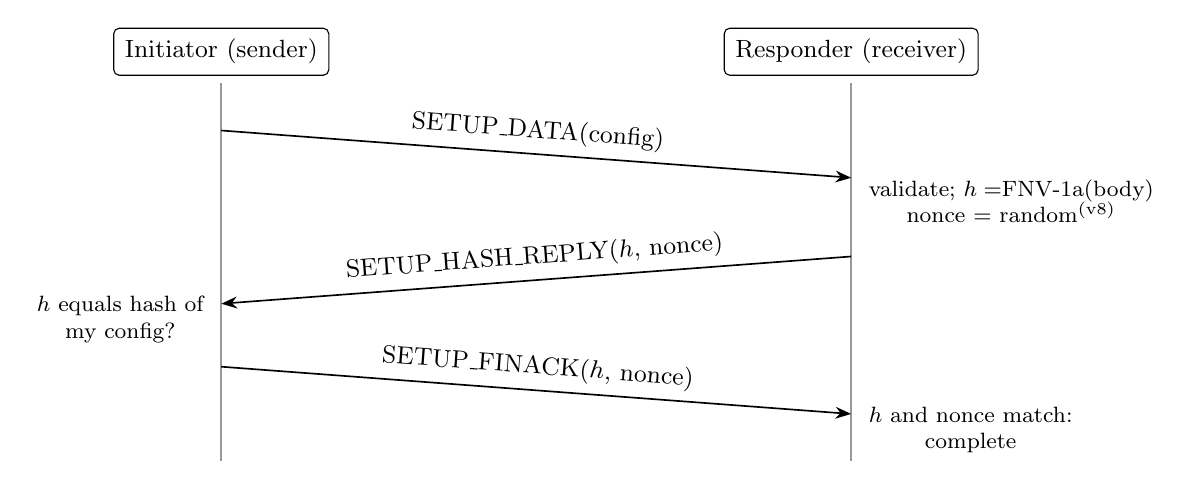
\begin{tikzpicture}[font=\small]
  \node[box] (i) at (0,0) {Initiator (sender)};
  \node[box] (r) at (8,0) {Responder (receiver)};
  \draw[thick,black!40] (0,-0.4) -- (0,-5.2); \draw[thick,black!40] (8,-0.4) -- (8,-5.2);
  \draw[msg] (0,-1) -- node[above,sloped] {SETUP\_DATA(config)} (8,-1.6);
  \node[lbl,right] at (8.1,-1.9) {validate; $h=$FNV-1a(body)\\nonce $=$ random\vviii};
  \draw[msg] (8,-2.6) -- node[above,sloped] {SETUP\_HASH\_REPLY($h$, nonce)} (0,-3.2);
  \node[lbl,left] at (-0.1,-3.4) {$h$ equals hash of\\my config?};
  \draw[msg] (0,-4.0) -- node[above,sloped] {SETUP\_FINACK($h$, nonce)} (8,-4.6);
  \node[lbl,right] at (8.1,-4.8) {$h$ and nonce match:\\complete};
\end{tikzpicture}}
\caption{The SETUP handshake. Retransmission timers on both sides recover any single loss.}\label{fig:setup}
\end{figure}

The responder echoes its \emph{own} hash of what it received rather than a simple ``ok''. A corrupted datagram
therefore produces a mismatched hash, so the handshake does not complete, whereas a corruptible boolean could
not detect that.

The responder nonce\vviii{} closes a replay attack: without it, a recorded SETUP\_DATA and SETUP\_FINACK pair
could be replayed later to complete a new handshake.

The responder also validates the offered configuration and ignores, without ever confirming, a SETUP that
violates any of these rules:
\begin{itemize}
  \item the protocol version must be its own;
  \item stream identifiers must be unique;
  \item block sizes must lie in 1--16,384;
  \item windows must lie in 1--1,024.
\end{itemize}
The multiplexed receiver additionally requires stream identifiers $0,\ldots,n-1$, because it indexes an array
with them. Both endpoints are pure state machines driven by received datagrams and timer calls.

\section{Hashing}

Two hash functions are provided:
\begin{itemize}
  \item \textbf{FNV-1a-64}~\cite{fnv}, a fast non-cryptographic hash. It serves as the SETUP checksum, as the
    file identity, and as the digest fallback in builds without cryptography.
  \item \textbf{SipHash-2-4}~\cite{siphash}, a keyed pseudorandom function. It computes the address-validation
    tokens\vviii, which must be unforgeable without the receiver's secret yet cheap enough to compute for every
    incoming StreamStart, including spoofed ones. SipHash was designed for exactly this kind of short keyed
    input, and it is available even in builds without wolfSSL.
\end{itemize}

\section{Session cryptography}\label{sec:crypto}

\paragraph{Why not one DTLS session per lane.} The obvious way to encrypt a sharded transfer is to give each
lane its own DTLS session. The implementation rejects this for two reasons, documented in
\code{session_crypto.hpp}:
\begin{itemize}
  \item A DTLS session owns record-layer state: sequence numbers, epoch, replay window and cipher state. That
    state cannot be shared across lanes without a mutex, which would serialise exactly the parallelism sharding
    creates.
  \item Writing through DTLS hands the socket to the library one record at a time, which destroys segmentation
    offload.
\end{itemize}
Instead, keys are derived once per session, and every lane encrypts independently with the same session key and
a nonce unique to the pair (lane, sequence number). Encrypted blocks remain fixed-size datagrams and pack into an
offload batch exactly as plaintext does. Fast QUIC implementations have the same shape: per-packet AEAD, followed
by batching of already-encrypted packets.

\paragraph{The lane cipher.} \code{LaneCipher} wraps one AES-256-GCM context. The tag is written directly after
the ciphertext so the datagram stays contiguous. A second initialisation is refused, because re-keying an
existing object is exactly how a (key, nonce) pair could repeat.

\paragraph{Key epochs\vviii.} One AES-GCM key should not protect an unbounded number of records; RFC~9001
applies a confidentiality limit of about $2^{23}$ packets~\cite{rfc9001}. Rather than adding rekeying messages,
each lane's key is derived deterministically from the session key, the lane and the epoch
$\mathit{seq}\gg22$, so both ends change keys at the same sequence number with nothing on the wire. A small
schedule keeps the two most recently used epochs, so that retransmissions from just before a boundary do not
force repeated derivations.

\paragraph{Control-plane authentication\vviii.} A \code{ControlAuth} object per lane and side appends and
verifies the GMAC trailer described in Section~\ref{sec:wirecrypto}, with its own key and a send counter that
starts at one. Replaying an old authentic control message is harmless by construction:
\begin{itemize}
  \item acknowledgement bases only ever move forward;
  \item an abort can only be replayed if one was genuinely sent.
\end{itemize}

\paragraph{Security properties.} The per-session random salt gives \emph{key freshness}: two sessions never
share a key. The pre-shared-key path does \emph{not} give forward secrecy. Anyone who records the traffic and
later obtains the key can decrypt it.

\paragraph{Digest and DTLS.} The digest used to verify resumed files is SHA-256 over the list of
per-64-MiB-segment SHA-256 values plus the file length, which allows the segments to be hashed in parallel.

A DTLS~1.2 wrapper with ECDHE-PSK cipher suites~\cite{rfc6347,rfc4279}, which does give forward secrecy, exists
as a standalone component and is tested, but no transport uses it yet. Version~8 made its debug copy of the wire
traffic opt-in.

\chapter{Bulk Transfer End to End}\label{ch:transfer}

The bulk-transfer API (\code{fuse/transfer.hpp}, implemented in \code{src/proto/transfer.cpp}) is the most
complete transport and the one that received the full version~8 hardening. This chapter follows a transfer
from configuration to completion.

\section{Interface and shape of a transfer}

The API consists of four blocking calls: \code{send_buffer}, \code{receive_buffer}, \code{send_file} and
\code{receive_file}. Each takes a \code{TransferConfig} (Appendix~\ref{app:config}) and returns a
\code{TransferStatus}. The receiver must be started first, because it has to be bound before the sender's
first message arrives.

The data is split into \code{lanes} equal shards, four by default. Lane $i$ is an independent reliable stream
with these properties:
\begin{itemize}
  \item it uses UDP port \code{base_port}$+i$ on the receiver, so the whole port range must be open;
  \item it has its own thread on the sender;
  \item it has its own reader thread on the receiver;
  \item it has its own sequence space, window, registry, congestion controller and keys.
\end{itemize}
A configuration whose last port would exceed 65,535 is rejected\vviii; before version~8 the sum wrapped around
to ports near zero.

On the receiver, a lane's reader thread does not write data itself. It hands each new block to one of $K$ writer
threads (\code{writer_threads}, two by default), or to a dedicated thread for retransmitted blocks, through
lock-free rings (Figure~\ref{fig:pipeline}). The writers decrypt and write each block directly to its final
position in the output. Only when a writer reports success does the reader admit the block to its window, so
every acknowledgement the sender sees covers bytes that are both authentic and already written.

\begin{figure}[H]
\centering
\fitwidth{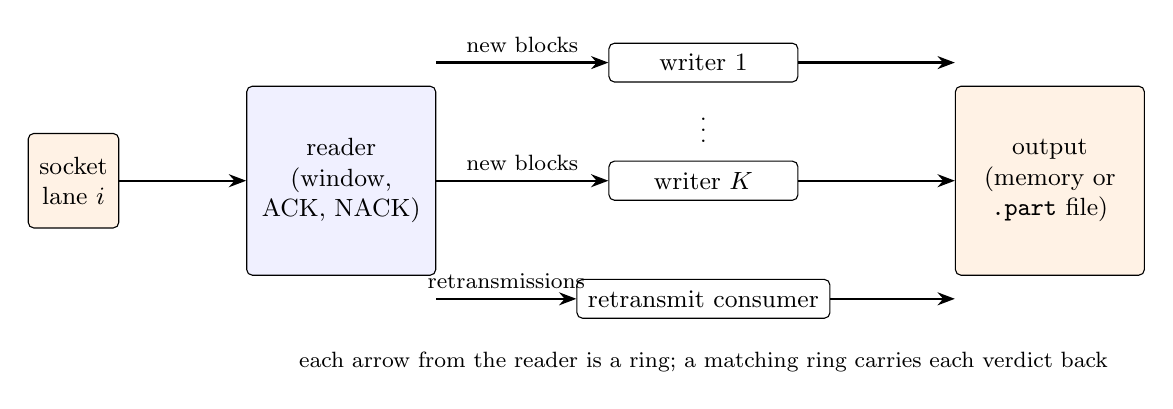
\begin{tikzpicture}[font=\small]
  \node[io,minimum height=1.2cm] (sock) at (0,0) {socket\\lane $i$};
  \node[core,minimum height=2.4cm,minimum width=2.4cm] (rd) at (3.4,0) {reader\\(window,\\ACK, NACK)};
  \node[box,minimum width=2.4cm] (w1) at (8,1.5) {writer 1};
  \node[lbl] at (8,0.75) {$\vdots$};
  \node[box,minimum width=2.4cm] (w2) at (8,0) {writer $K$};
  \node[box,minimum width=2.4cm] (rt) at (8,-1.5) {retransmit consumer};
  \node[io,minimum height=2.4cm,minimum width=2.4cm] (sink) at (12.4,0) {output\\(memory or\\\texttt{.part} file)};
  \draw[arr] (sock) -- (rd);
  \draw[arr] (rd.east|-w1) -- node[above,lbl]{new blocks} (w1.west);
  \draw[arr] (rd.east|-w2) -- node[above,lbl]{new blocks} (w2.west);
  \draw[arr] (rd.east|-rt) -- node[above,lbl]{retransmissions} (rt.west);
  \draw[arr] (w1.east) -- (sink.west|-w1); \draw[arr] (w2.east) -- (sink.west|-w2); \draw[arr] (rt.east) -- (sink.west|-rt);
  \node[lbl,below=3mm of rt] {each arrow from the reader is a ring; a matching ring carries each verdict back};
\end{tikzpicture}}
\caption{Receive pipeline of one lane. Solid arrows carry datagrams and dashed arrows carry verdicts back.
Every ring has one producer and one consumer, so no mutex is needed.}\label{fig:pipeline}
\end{figure}

New blocks are routed to writer $\lfloor \mathit{seq}/64\rfloor \bmod K$: whole runs of 64 consecutive blocks go
to the same writer, which can then write each run with a single \code{pwritev}. Round-robin routing
($\mathit{seq}\bmod K$) left every writer's blocks non-adjacent, and was measured to be two to four times slower
on a real disk. A full ring never blocks the reader: the datagram is dropped and recovered by the normal loss
recovery.

\section{Opening a lane}\label{sec:handshake}

Figure~\ref{fig:handshake} shows how a lane is opened. The sender draws a random 64-bit lane nonce from a
secure source and sends a StreamStart. Under a pre-shared key, the StreamStart carries the session salt and the
control trailer.

\begin{figure}[H]
\centering
\fitwidth{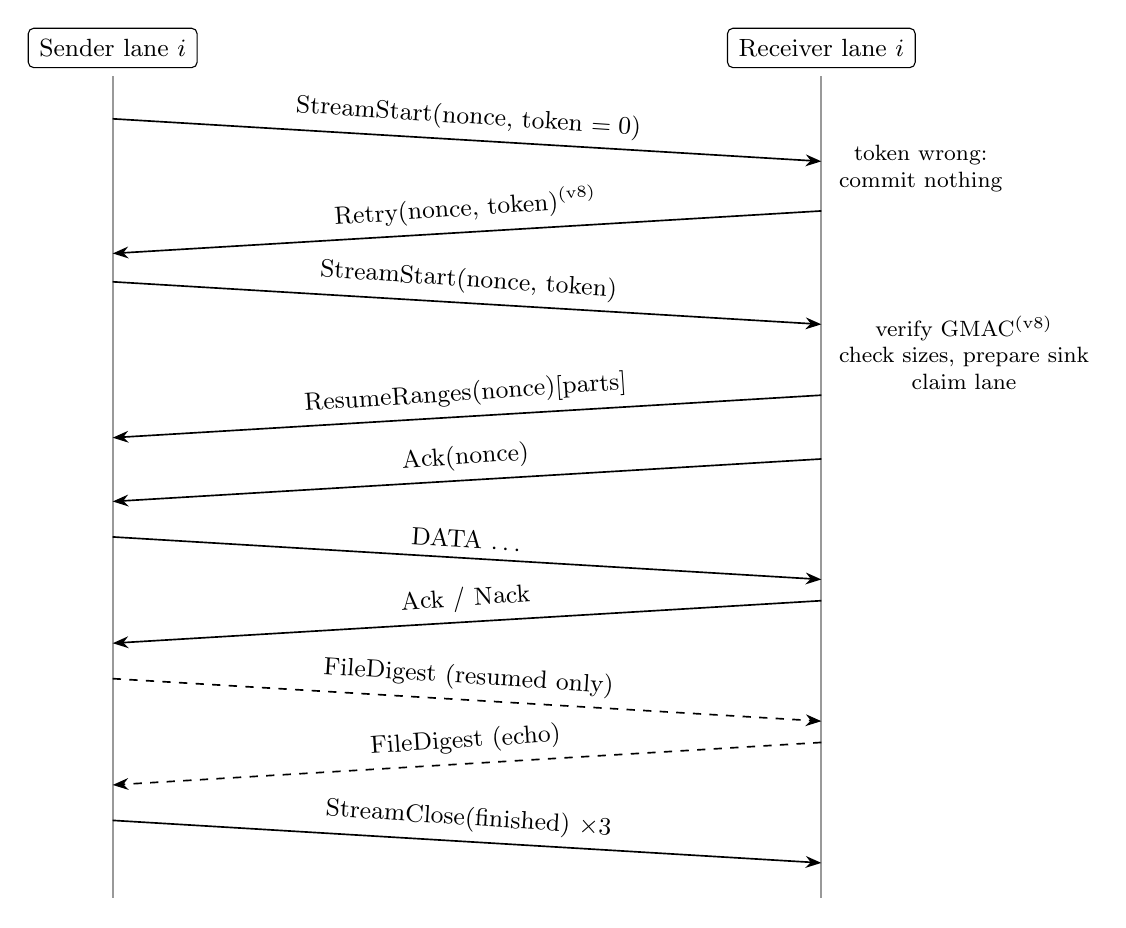
\begin{tikzpicture}[font=\small,yscale=0.9]
  \node[box] at (0,0.4) {Sender lane $i$};
  \node[box] at (9,0.4) {Receiver lane $i$};
  \draw[thick,black!40] (0,0) -- (0,-11.6); \draw[thick,black!40] (9,0) -- (9,-11.6);
  \draw[msg] (0,-0.6) -- node[above,sloped]{StreamStart(nonce, token $=0$)} (9,-1.2);
  \node[lbl,right] at (9.1,-1.3) {token wrong:\\commit nothing};
  \draw[msg] (9,-1.9) -- node[above,sloped]{Retry(nonce, token)\vviii} (0,-2.5);
  \draw[msg] (0,-2.9) -- node[above,sloped]{StreamStart(nonce, token)} (9,-3.5);
  \node[lbl,right] at (9.1,-3.9) {verify GMAC\vviii\\check sizes, prepare sink\\claim lane};
  \draw[msg] (9,-4.5) -- node[above,sloped]{ResumeRanges(nonce)[parts]} (0,-5.1);
  \draw[msg] (9,-5.4) -- node[above,sloped]{Ack(nonce)} (0,-6.0);
  \draw[msg] (0,-6.5) -- node[above,sloped]{DATA \ldots} (9,-7.1);
  \draw[msg] (9,-7.4) -- node[above,sloped]{Ack / Nack} (0,-8.0);
  \draw[msg,dashed] (0,-8.5) -- node[above,sloped]{FileDigest (resumed only)} (9,-9.1);
  \draw[msg,dashed] (9,-9.4) -- node[above,sloped]{FileDigest (echo)} (0,-10.0);
  \draw[msg] (0,-10.5) -- node[above,sloped]{StreamClose(finished) $\times3$} (9,-11.1);
\end{tikzpicture}}
\caption{The life of a lane. Every reply carries the lane nonce; under a pre-shared key every message except
Retry carries a control trailer.}\label{fig:handshake}
\end{figure}

\paragraph{Address validation\vviii.} On receiving a StreamStart, the receiver first computes
\[
\mathit{token}=\mathrm{SipHash\text{-}2\text{-}4}_{s}(\mathit{family}\,\|\,\mathit{port}\,\|\,\mathit{address}\,\|\,\mathit{nonce}),
\]
where $s$ is a 128-bit secret held only by this receiver lane. If the StreamStart does not carry this token, the
receiver replies with a 20-byte Retry and does nothing else. It allocates nothing, claims nothing and sends
nothing larger than the request. Only a sender that genuinely receives at its claimed address can echo the
token. A spoofed StreamStart can therefore neither take over the lane nor turn the receiver into an amplifier
aimed at a victim. This is the same mechanism as QUIC's Retry~\cite{rfc9000}.

\paragraph{Key confirmation\vviii.} When a StreamStart with a valid token arrives and the lane has no session
yet, the receiver authenticates it before allocating anything. It derives the session key from its own
pre-shared key and the StreamStart's salt, creates a trial control authenticator, and verifies the trailer. Two
outcomes are possible:
\begin{itemize}
  \item \emph{Verification fails.} This happens when the keys differ, when only one side has a key, or when a
    plaintext receiver meets an encrypting sender. The receiver answers, unauthenticated and at most once per
    100~ms, with StreamClose(reason~2). The sender then reports \code{AuthFailed} immediately, instead of after
    twenty failed data blocks or a timeout.
  \item \emph{Verification succeeds.} The receiver validates the sizes in an order that cannot overflow, namely
    $\mathit{total\_bytes}\le\mathit{file\_total}$ and
    $\mathit{base\_offset}\le\mathit{file\_total}-\mathit{total\_bytes}$. The first lane to succeed then sizes
    the output with an atomic compare-and-swap, and every other lane must agree on the total. If the claimed
    size cannot be allocated, the receiver fails with \code{ResourceLimit}.
\end{itemize}

\paragraph{Answer and retries.} The receiver then records the lane nonce and the sender's address, computes the
byte ranges of the lane it still needs (all of it, unless it is resuming), and sends them as ResumeRanges
followed by Ack messages. The sender considers the handshake complete only once it has an Ack and every
ResumeRanges part carrying its nonce. It retries its StreamStart with exponential backoff from 1~ms to 200~ms,
bounded by \code{connect_timeout_ms} (10~s by default); a retried StreamStart with the right nonce makes the
receiver re-send its answer. The ranges are checked for order, overlap and bounds before use, and an
inconsistent answer makes the sender send the whole lane instead.

\section{The sender's main loop}\label{sec:sendloop}

After the handshake the sender lane runs one loop until every byte is acknowledged or the lane gives up. Each
iteration performs five steps.

\begin{enumerate}
  \item \textbf{Stop checks.} The loop first handles user cancellation and the shared \code{stop_all} flag, which
    is set when a sibling lane has heard the peer abort.
  \item \textbf{Window computation.} It advances the congestion controller and computes the bytes it may have in
    flight:
    \[
    \mathit{window\_bytes}=\min\bigl(\max(4,\mathit{cwnd})\cdot\mathit{base\_block},\;\max(4,\mathit{rwnd})\cdot\mathit{block}\bigr).
    \]
    Here $\mathit{cwnd}$ is counted in units of the \emph{configured} block size\vviii{} and $\mathit{rwnd}$ is
    the receiver's advertised window\vviii. The floor of four keeps a zero window from wedging the flow.
  \item \textbf{Sending a batch.} If there is room in the window and in the 1,024-slot registry, and the pacing
    time has passed, the sender builds a batch:
    \begin{itemize}
      \item It stores each block in the registry, seals it, encodes the DATA datagram into a staging buffer, and
        sends the batch with segmentation offload, falling back to individual sends.
      \item The batch is limited by the offload budget (about 60~KB), the registry, the window and a burst cap.
        The cap is 16 datagrams once the path has a real round-trip time (above 1~ms), because a 64-datagram
        line-rate burst overflows shallow router buffers.
      \item The next batch is paced (Section~\ref{sec:cc}).
    \end{itemize}
  \item \textbf{Reading control traffic.} It drains up to 64 control datagrams. Under a pre-shared key, any
    datagram without a valid trailer is discarded before it is even parsed. Otherwise:
    \begin{itemize}
      \item an \emph{Ack} with the right nonce is applied with \code{apply_ack}, its \code{rwnd} recorded, and a
        new echoed send time fed to the RTT estimator;
      \item a \emph{Nack} marks a loss in the controller and resends each listed block;
      \item a \emph{StreamClose(aborted)} ends the lane with \code{PeerAborted};
      \item a \emph{PathChallenge} is answered, and a \emph{PathResponse} completes a pending path validation
        (Section~\ref{sec:path}).
    \end{itemize}
  \item \textbf{Timeout and adaptation.} It runs the retransmission timeout and the block-size adaptation
    (Sections~\ref{sec:recovery} and~\ref{sec:blocksize}), and gives up with \code{Timeout} if no acknowledgement
    has confirmed new data for \code{timeout_ms}.
\end{enumerate}

\paragraph{RTT samples from repeated echoes.} A repeated echo is never treated as a new RTT sample. The receiver
only updates its echoed send time when a new highest block arrives, so its periodic acknowledgements repeat the
same value. Counting each repeat as a fresh sample manufactured an ever-growing fake RTT whenever the sender was
stalled on a gap, which stretched the timer exactly when it needed to stay responsive.

\paragraph{The empty case.} A lane with nothing to send still needs a completion signal: an empty send, an
uneven split, or a resumed lane that is already complete. The lane sends a single empty block marked LastBlock.

\section{The life of one packet}\label{sec:life}

To make the pieces concrete, we follow one encrypted block, number 4,711 of lane~2, from the sender's memory to
the receiver's disk.

\begin{enumerate}
  \item \textbf{Admission.} The lane's congestion and receive windows have room and the pacing time has passed.
    The block's bytes are copied into registry slot $4711 \bmod 1024$, together with their offset, length and
    flags.
  \item \textbf{Key and nonce.} The key schedule selects the cipher for epoch $4711\gg22=0$. The nonce is
    $\langle 2, 4711, \text{0x0000}\rangle$, and the AAD is $\langle 2, 4711, \mathit{offset}, \mathit{flags}
    \wedge\lnot\text{0x01}\rangle$.
  \item \textbf{Sealing.} AES-256-GCM encrypts the payload into a scratch buffer and appends the tag; if sealing
    fails, the batch stops.
  \item \textbf{Framing.} The datagram is the outer header, the 21-byte block header with
    \code{payload_len} including the tag, the send time plus the lane's secret offset, and the ciphertext.
  \item \textbf{Transmission.} It joins up to 15 other datagrams in the staging buffer, and the batch leaves in
    one \code{sendmsg} with \code{UDP_SEGMENT}. The kernel splits the buffer into individual datagrams.
  \item \textbf{Reception.} On the receiver, the lane's reader collects it with up to 63 others in one
    \code{recvmmsg}, peeks at the type, and decodes the header. It discards the block if the block is below the
    base, beyond the window, already received, or currently held by a writer. Otherwise it copies the datagram
    into the ring of writer $\lfloor4711/64\rfloor\bmod K$.
  \item \textbf{Decryption and write.} The writer selects its own cipher for the lane and epoch, rebuilds the
    AAD, and opens the block. On success it checks that
    $\mathit{offset}\le\mathit{lane\_total}$ and $\mathit{len}\le\mathit{lane\_total}-\mathit{offset}$, merges
    the block with any adjacent blocks in its batch, and writes the run with one \code{pwritev} at
    $\mathit{lane\_base}+\mathit{offset}$. It posts the verdict to the reader's completion ring.
  \item \textbf{Admission to the window.} The reader collects the verdict and calls \code{on_receive}. The bit
    for 4,711 is set; if it was the first gap, the base slides forward. If the block came from a new source
    address, a path challenge is sent there (Section~\ref{sec:path}).
  \item \textbf{Acknowledgement.} After eight newly delivered blocks, or 200~\textmu s, or a window update, the
    reader sends an Ack. The Ack carries the new base, the bitmask, the echoed send time, the nonce and the
    current receive window, and is signed with the control trailer.
  \item \textbf{Release.} The sender verifies the trailer and applies the Ack, releasing slot $4711\bmod 1024$.
    The block's bytes now count towards progress, and the window may grow.
\end{enumerate}

\section{Loss recovery}\label{sec:recovery}

Fuse recovers losses through three cooperating mechanisms.

\paragraph{Negative acknowledgements.} The receiver reports gaps that have persisted beyond a reorder delay and
were not reported within a re-NACK interval. Both intervals scale with the receiver's own estimate of the RTT:
\begin{itemize}
  \item the reorder delay is half the RTT, clamped to 1--100~ms;
  \item the re-NACK interval is 1.5 times the RTT, clamped to 20--500~ms;
  \item before any estimate exists, conservative wide-area defaults of 3~ms and 40~ms apply.
\end{itemize}
The receiver measures the RTT purely on its own clock, as the delay between sending a NACK and receiving the
retransmission it requested, so no comparison between the two hosts' clocks is needed. Scaling matters: with
fixed loopback-tight values, a wide-area path received a duplicate NACK every few milliseconds while the
retransmission was still 50~ms away.

\paragraph{Selective acknowledgement\vviii.} Every Ack confirms blocks above the base through its bitmask, so a
NACK or timeout never resends a block the receiver already holds.

\paragraph{Retransmission timeout\vviii.} If the base has not advanced for one RTO (Section~\ref{sec:cc}), the
sender resends the base and up to seven further \emph{known holes}: unacknowledged blocks below
\code{received_end}, the highest block the receiver is known to hold. After a burst loss, the rest of the burst
is therefore repaired in one timeout rather than one timeout per block, without resending blocks that are merely
in flight. A send that the kernel refuses, for example because the socket buffer is full, does not count as
progress; otherwise the block would never be retransmitted and the transfer would stall.

\section{Flow control}\label{sec:flow}

Before version~8 there was no flow control. A receiver whose writers fell behind a fast sender (because of a
slow disk, say) silently dropped blocks at its full rings. The sender interpreted the losses as network
congestion: NACKs, retransmissions and a halved window.

Now each Ack advertises the receive window, which is the free space in the lane's writer rings plus the blocks
already handed over but not yet written, capped at 1,024. The sender keeps its bytes in flight within it. When
the advertised window was low (below a quarter of the maximum) and has since at least doubled, the receiver
sends an Ack immediately as a \emph{window update}. Without the update, a sender that paused for the receiver
would sit idle until the next periodic acknowledgement. This is the behaviour that removed a throughput
regression found while the feature was being developed.

\section{Adaptive block size and the MTU}\label{sec:blocksize}

The sender starts with the configured block size, 1,200 bytes by default, and doubles it after eight batches
in a row that were confirmed by acknowledgements, up to a \emph{growth ceiling}\vviii. Any loss returns the
block size to the configured value. Growth is counted in acknowledged batches rather than loop iterations, which
can accumulate many times within one round trip, before any acknowledgement could have arrived.

The growth ceiling is computed from the kernel's route MTU:
\[
\mathit{ceiling}=\min\bigl(\mathit{block\_ceiling},\;\mathit{mtu}-\mathit{ip\_udp}-31-\mathit{tag}\bigr),
\]
and is never below the starting size. An unknown MTU means no growth at all. On loopback, which reports a
64~KiB MTU, blocks may still grow to 16~KiB; on an ordinary 1,500-byte path they stop at about 1,450 bytes.
Before version~8, blocks grew to 16~KiB on any path. Above the MTU every such datagram is fragmented, and losing
one fragment loses the whole datagram.

On top of the MTU bound, a loss that occurs soon after a growth step makes the previous size the new ceiling,
so on a path that drops large datagrams the size settles instead of oscillating. In the spirit of
DPLPMTUD~\cite{rfc8899}, the larger size is probed again after a clean stretch, and that stretch doubles after
each failed probe, up to 4,096 acknowledged batches. One transient loss therefore does not cap the lane
permanently.

The congestion window counts units of the \emph{configured} block size. Its cap is the number of units that
1,024 blocks of the largest permitted size would occupy, so a long fat path can still be filled, but only by
earning the window through slow start and additive increase. Previously the window counted blocks of whatever
size they had grown to, so the same window could hold up to 13 times as many bytes. Slow start starts from 128
units, about the 150~KB a lane used to begin with.

\section{Path validation}\label{sec:path}

A receiver whose peer is behind a NAT may see the sender's source address change in the middle of a transfer
when the NAT rebinds. Before version~8, the bulk transfer simply re-anchored its peer address to the source of
any accepted block. An attacker could then redirect a lane's acknowledgements, or reflect traffic at a third
party, with a single spoofed datagram.

Now, when authentic session traffic arrives from a new source, the side that sees it sends a PathChallenge with
a fresh random 64-bit value to that source. It switches its peer address only when a matching PathResponse comes
back \emph{from that source}. One candidate is validated at a time, and challenges are resent at most every
50~ms. Data from the new source is accepted in the meantime, so a genuine rebinding costs no throughput. The
mechanism is symmetric: the sender validates a new source of Acks in the same way.

\section{Finishing a lane}

The receiver knows a lane is complete when it has seen the block carrying LastBlock and the base has moved past
it. The flag is trusted only after the block has authenticated.

The receiver does not exit at once. It keeps sending acknowledgements on its normal schedule in case its last
ones were lost, and it leaves at the first of three events:
\begin{itemize}
  \item the sender's StreamClose(finished) arrives;
  \item the sender has been silent for 400~ms;
  \item 1.5~s have passed since completion.
\end{itemize}
It then sends eight final acknowledgements. The lane's reported duration ends at completion rather than after
this linger, so throughput figures are not diluted.

For a resumed transfer, lane~0 also waits for the sender's whole-file digest. The sender computes the digest in a
background thread that starts right after the handshake, overlapped with sending the missing data. It re-sends
the digest every 50~ms until the receiver echoes it, and then sends StreamClose(finished) three times.

\section{State machines of the two lane roles}

Figures~\ref{fig:sendfsm} and~\ref{fig:recvfsm} summarise the behaviour described above.

\begin{figure}[H]
\centering
\fitwidth{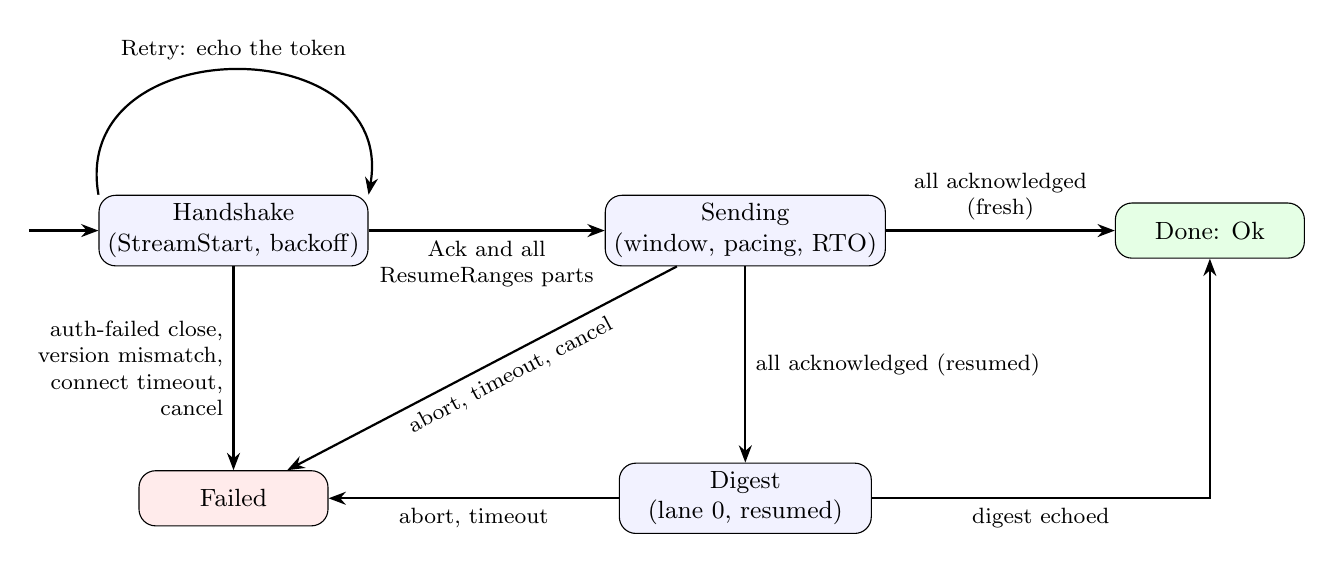
\begin{tikzpicture}[>={Stealth[length=2.2mm]},font=\small]
  \node[st,minimum width=3.2cm] (hs) at (0,0) {Handshake\\(StreamStart, backoff)};
  \node[st,minimum width=3.2cm] (sending) at (6.5,0) {Sending\\(window, pacing, RTO)};
  \node[st,minimum width=2.4cm,fill=green!10] (ok) at (12.4,0) {Done: Ok};
  \node[st,minimum width=3.2cm] (digest) at (6.5,-3.4) {Digest\\(lane 0, resumed)};
  \node[st,minimum width=2.4cm,fill=red!8] (fail) at (0,-3.4) {Failed};
  \draw[->,thick] (-2.6,0) -- (hs);
  \draw[->,thick] (hs) -- node[lbl,below]{Ack and all\\ResumeRanges parts} (sending);
  \draw[->,thick] (hs.north west) to[out=100,in=80,looseness=1.6] node[lbl,above]{Retry: echo the token} (hs.north east);
  \draw[->,thick] (hs) -- node[lbl,left,align=right]{auth-failed close,\\version mismatch,\\connect timeout,\\cancel} (fail);
  \draw[->,thick] (sending) -- node[lbl,above]{all acknowledged\\(fresh)} (ok);
  \draw[->,thick] (sending) -- node[lbl,right]{all acknowledged (resumed)} (digest);
  \draw[->,thick] (digest) -| node[lbl,below,pos=0.25]{digest echoed} (ok);
  \draw[->,thick] (sending) -- node[lbl,below,sloped,pos=0.45]{abort, timeout, cancel} (fail);
  \draw[->,thick] (digest) -- node[lbl,below]{abort, timeout} (fail);
\end{tikzpicture}}
\caption{Sender lane. Every transition to \emph{Failed} except a received abort sends StreamClose(aborted) to the peer.}\label{fig:sendfsm}
\end{figure}

\begin{figure}[H]
\centering
\fitwidth{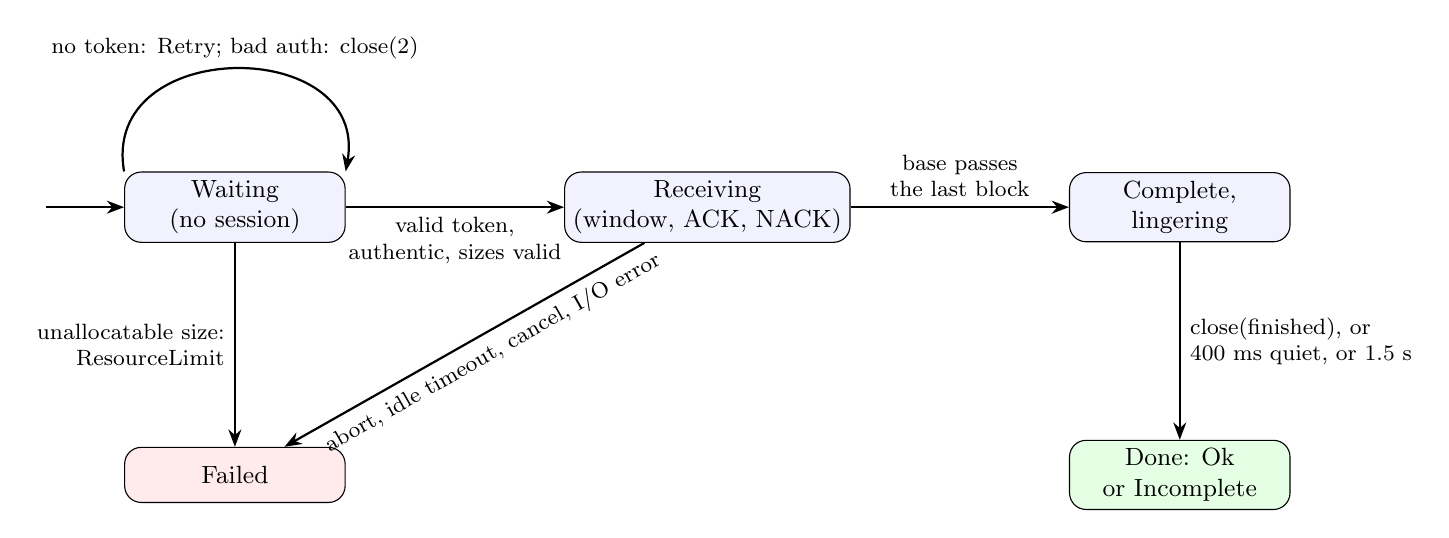
\begin{tikzpicture}[>={Stealth[length=2.2mm]},font=\small]
  \node[st,minimum width=2.8cm] (wait) at (0,0) {Waiting\\(no session)};
  \node[st,minimum width=3.2cm] (recv) at (6,0) {Receiving\\(window, ACK, NACK)};
  \node[st,minimum width=2.8cm] (linger) at (12,0) {Complete,\\lingering};
  \node[st,minimum width=2.8cm,fill=green!10] (ok) at (12,-3.4) {Done: Ok\\or Incomplete};
  \node[st,minimum width=2.8cm,fill=red!8] (fail) at (0,-3.4) {Failed};
  \draw[->,thick] (-2.4,0) -- (wait);
  \draw[->,thick] (wait.north west) to[out=100,in=80,looseness=1.6] node[lbl,above]{no token: Retry; bad auth: close(2)} (wait.north east);
  \draw[->,thick] (wait) -- node[lbl,below]{valid token,\\authentic, sizes valid} (recv);
  \draw[->,thick] (recv) -- node[lbl,above]{base passes\\the last block} (linger);
  \draw[->,thick] (linger) -- node[lbl,right,align=left]{close(finished), or\\400 ms quiet, or 1.5 s} (ok);
  \draw[->,thick] (wait) -- node[lbl,left,align=right]{unallocatable size:\\ResourceLimit} (fail);
  \draw[->,thick] (recv) -- node[lbl,below,sloped,pos=0.45]{abort, idle timeout, cancel, I/O error} (fail);
\end{tikzpicture}}
\caption{Receiver lane. The final status is classified as \texttt{AuthFailed} if most blocks failed authentication.}\label{fig:recvfsm}
\end{figure}

\section{Cancellation, abort, timeout and combining statuses}

\paragraph{Cancellation.} \code{TransferConfig::cancel} is an atomic flag that every lane polls. Its loop
cadence is bounded by short socket timeouts, at most 20~ms on the receiver. When the flag is set, a lane sends
StreamClose(aborted) three times and returns \code{Cancelled}, and its siblings stop as well. The peer returns
\code{PeerAborted} instead of waiting out its timeout.

\paragraph{Aborts before a session exists.} Under plaintext, an abort is accepted with any nonce, so a sender
cancelled before its StreamStart arrived can still say ``I am not coming''. Under a pre-shared key, such an abort
cannot be verified and is ignored.

\paragraph{Timeouts.} The receiver gives up when no datagram has arrived for \code{timeout_ms} plus one second.
The sender gives up when no acknowledgement has confirmed new data for \code{timeout_ms}.

\paragraph{Detecting an active attack.} If at least 20 blocks have been seen and more than half of them failed
authentication, the receiver reports \code{AuthFailed}. An active tampering attack fails most blocks, which is
distinguishable from ordinary loss, and the caller should learn of it as such.

\paragraph{Combining lane statuses.} The call's result is the most severe lane status, so that the caller sees
the most actionable problem rather than whichever lane finished last. The ranking, from least to most severe,
is:
\begin{quote}\small
Ok $<$ Incomplete $<$ Timeout $<$ PeerAborted $<$ Cancelled $<$ AuthFailed $<$ VerifyFailed $<$ ResourceLimit
$<$ IoError $<$ SocketError $<$ VersionMismatch $<$ ConfigError, Unsupported.
\end{quote}

\section{Resumable file reception}\label{sec:resume}

\code{receive_file} writes into \code{<path>.part} and renames it over \code{<path>} only after every byte has
arrived and been synchronised to disk, so the destination file is always either untouched or complete. Behind
the data, the \code{.part} file carries a trailer
\[
[\,\text{data}\,][\,\text{bitmap: one bit per chunk}\,][\,\mathit{file\_id},\mathit{total},\mathit{chunk},\mathit{nchunks},\mathit{checksum},\text{``FUSERSM1''}\,].
\]
Chunks are 64~KiB, doubled for very large files until there are at most $2^{23}$ of them. They are used rather
than sequence numbers because the mapping from sequence number to offset changes with the block size, both
during and between sessions. The trailer is rewritten every \code{resume_checkpoint_ms} (one second) and
whenever a transfer ends without completing.

A later \code{receive_file} of the same file adopts the partial copy. Its StreamStart must carry the same
\code{file_id} and size; the receiver then asks only for the missing chunks, merging the closest ranges if the
list would exceed 4,096. At the end it verifies the whole file against the sender's digest. On a mismatch it
reports \code{VerifyFailed} and \emph{discards} the copy, since another resume would fail the same way.

The file identity hashes the file's name, size, modification time, inode change time, inode number and
device\vviii. Before version~8 it used only name, size and modification time, which missed a file rewritten in
place with its modification time set back (by \code{touch -r} or a restore tool); a resume would then have
stitched stale bytes into the result. The inode change time cannot be set back by user code.

\section{Timers}

\begin{table}[H]
\centering\small
\caption{Every timer of the bulk transfer.}\label{tab:timers}
\begin{tabularx}{\linewidth}{>{\raggedright\arraybackslash}p{4.4cm}>{\raggedright\arraybackslash}p{3.6cm}X}
\toprule
\textbf{Timer} & \textbf{Value} & \textbf{Purpose} \\
\midrule
StreamStart retry & 1~ms doubling to 200~ms & handshake on any path RTT \\
Connect timeout & \code{connect_timeout_ms} (10~s) & fail fast if no receiver \\
No-progress timeout & \code{timeout_ms} (120~s) & sender: no acknowledged progress \\
Receiver idle limit & \code{timeout_ms} $+$ 1~s & receiver: no datagrams at all \\
Periodic ACK & every 8 blocks or 200~\textmu s & feedback cadence \\
Quiet ACK limit & 3 to a silent peer\vviii & no endless reflection \\
Reorder delay & RTT/2, 1--100~ms (3~ms initially) & late is not lost \\
Re-NACK interval & 1.5 RTT, 20--500~ms (40~ms initially) & no duplicate repair \\
RTO & Section~\ref{sec:cc}, 5~ms--1~s, backoff $\le 2^6$ & tail and burst losses \\
Path challenge resend & 50~ms\vviii & validate a new address \\
Version / auth reply limit & 100~ms\vviii & no reflection amplifier \\
Digest resend & 50~ms & resumed transfers \\
Completion linger & close, 400~ms quiet, or 1.5~s & lost final ACKs \\
Resume checkpoint & \code{resume_checkpoint_ms} (1~s) & crash-safe progress \\
\bottomrule
\end{tabularx}
\end{table}

\chapter{The Socket-Style SDK and the Multiplexed Transfer}\label{ch:sdkmux}
\chaptermark{SDK and Multiplexed Transfer}

\section{The socket-style SDK}\label{sec:sdk}

\subsection{Contract}

\code{fuse/sdk.h} is a C API that will look familiar to anyone who has written a TCP server:
\code{fuse_listen}, \code{fuse_accept}, \code{fuse_connect}, \code{fuse_send}, \code{fuse_recv} and
\code{fuse_close}. Its semantics differ from TCP in four ways that a programmer must know:
\begin{itemize}
  \item \textbf{Messages, not a byte stream.} What one \code{fuse_send} delivers, exactly one \code{fuse_recv}
    returns. Boundaries are preserved, as with \code{SOCK_SEQPACKET}, so there is no length prefixing and no
    partial read.
  \item \textbf{Reliable and ordered over UDP.} Loss is repaired underneath; the application sees either the
    whole message or an error.
  \item \textbf{Completion means delivery.} \code{fuse_send} returns once the peer has acknowledged the message,
    not when it has been queued locally.
  \item \textbf{Optional encryption.} The same pre-shared key on both ends seals every message with AES-256-GCM.
\end{itemize}
A message may be up to 64~MiB. A connection may be used from several threads, typically one sending and one
receiving, and serialises its own operations internally.

\subsection{Connecting: one listen port, a fresh port per connection}

Figure~\ref{fig:sdkconnect} shows how a connection is established:
\begin{enumerate}
  \item The client sends HELLO($\mathit{salt}_c$, challenge) to the server's well-known port.
  \item The server allocates a connection object, a fresh ephemeral socket and a pump thread.
  \item It replies with HELLO\_ACK($\mathit{salt}_s$, proof) \emph{from the new socket}, and the client adopts
    that source address as its peer.
\end{enumerate}
As in TFTP~\cite{rfc1350}, a single open port serves any number of connections without connection identifiers.

The session key is derived with HKDF from the pre-shared key and the concatenation
$\mathit{salt}_c\,\|\,\mathit{salt}_s$, so that neither side alone determines it. The server's salt was added
in version~4 after a subtle problem was found. With only the client's salt, a HELLO retried before its first
reply arrived could create two live connections with the same key, and both would start their sequence numbers
at zero: an AES-GCM (key, nonce) collision. The proof is the client's challenge sealed under the session key, and
it demonstrates that the server holds the key. The two directions of a connection use different stream
identifiers (0 for client to server, 1 for server to client), and because the stream identifier is part of the
nonce, the directions never share one.

\begin{figure}[H]
\centering
\fitwidth{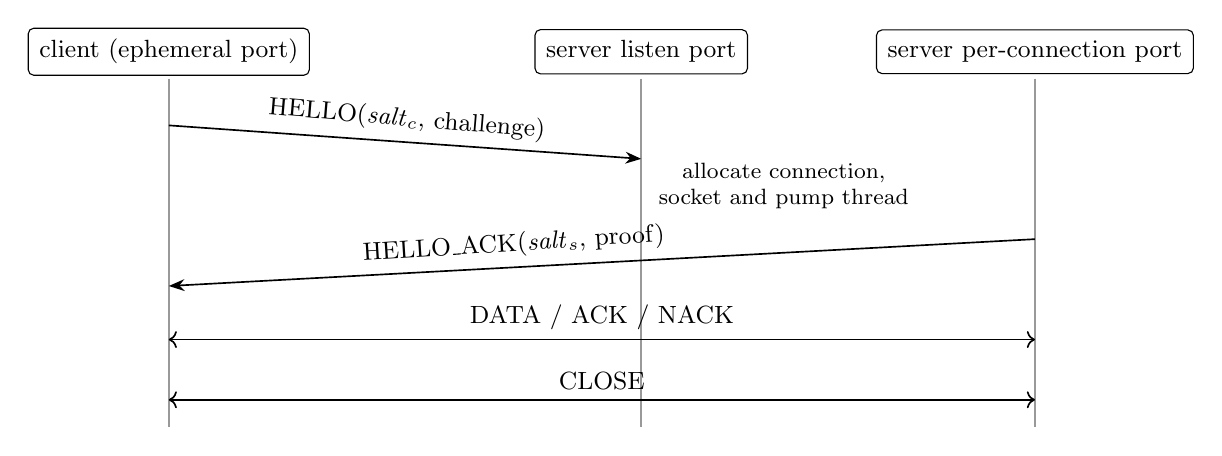
\begin{tikzpicture}[font=\small,yscale=0.85]
  \node[box] at (0,0.4) {client (ephemeral port)};
  \node[box] at (6,0.4) {server listen port};
  \node[box] at (11,0.4) {server per-connection port};
  \foreach \x in {0,6,11} \draw[thick,black!40] (\x,0) -- (\x,-5.2);
  \draw[msg] (0,-0.7) -- node[above,sloped]{HELLO($\mathit{salt}_c$, challenge)} (6,-1.2);
  \node[lbl,right] at (6.1,-1.6) {allocate connection,\\socket and pump thread};
  \draw[msg] (11,-2.4) -- node[above,sloped,pos=0.6]{HELLO\_ACK($\mathit{salt}_s$, proof)} (0,-3.1);
  \draw[msg,<->] (0,-3.9) -- node[above]{DATA / ACK / NACK} (11,-3.9);
  \draw[msg,<->] (0,-4.8) -- node[above]{CLOSE} (11,-4.8);
\end{tikzpicture}}
\caption{SDK connection establishment. The client adopts the HELLO\_ACK's source address as its peer.}\label{fig:sdkconnect}
\end{figure}

\subsection{Inside a connection}

Each connection has one UDP socket, one peer and a background \emph{pump} thread that does all the wire work:
receiving, reassembling, acknowledging and retransmitting. Because of the pump, a blocked \code{fuse_recv} still
sends acknowledgements and a blocked \code{fuse_send} still repairs loss. The application calls are thin. They
hand a message to the pump, or take one from it, through a mutex and a condition variable.

\paragraph{Framing.} A message is carried as a run of DATA blocks whose \code{offset} is the byte position
within the message, with LastBlock on the final one. The receiver knows the message is complete when its window
base passes the final block, so a truncated message can never reach the application. Block $\mathit{seq}$ of a
message must sit exactly at offset $(\mathit{seq}-\mathit{first\_seq})\times1200$, so a forged block cannot claim
an offset near 64~MiB and force a large allocation (R8).

\paragraph{Backpressure.} Completed messages wait in an inbox capped at 256~MiB of undelivered data. When the cap
is reached, new blocks are not admitted, and the sender's own retransmission logic stalls until the application
drains the inbox.

\paragraph{Liveness\vviii.} A connection that has sent nothing for one second sends a HEARTBEAT. A peer that
has sent nothing at all (no data and no authentic control message) for $\max(\mathit{timeout\_ms},3\,\mathrm{s})$
is declared lost, and blocked calls return \code{FUSE_ERR_TIMEOUT}.

\paragraph{Closing.} \code{fuse_close} sends CLOSE and stops the pump. The connection is reference-counted by
the application threads inside \code{fuse_send} and \code{fuse_recv}, and the last one to leave frees it, so
closing can never free a connection another thread is still using.

\subsection{Security}

The SDK was left out of the first version~8 pass and brought up to the same standard by the second. It now
shares the bulk transfer's protections:
\begin{itemize}
  \item retransmissions are sealed with the retransmission bit outside the AAD, which removes the nonce-reuse
    flaw (Section~\ref{sec:nonce});
  \item data keys rotate every $2^{22}$ blocks, and blocks outside the receive window are dropped before
    decryption, so forged far-off sequence numbers cannot force key derivations (R7);
  \item under a pre-shared key, ACK, NACK, CLOSE, HEARTBEAT and the path probes are signed and replay-checked;
    in plaintext they are acted on only from the peer's current address, where previously a two-byte CLOSE from
    anywhere ended a connection;
  \item the peer address moves only after the new source answers a path challenge, using the shared
    \code{PathValidator};
  \item binary keys with zero bytes are supported through \code{pre_shared_key_len}.
\end{itemize}

\noindent Three issues remain open, listed in Table~\ref{tab:open}:
\begin{itemize}
  \item the server still allocates a connection, a socket and a thread for every HELLO before the client
    proves anything; heartbeats now bound how long such a connection lives;
  \item the SDK is stop-and-wait per message;
  \item its registry uses about 17~MB per connection, because each slot embeds a 16~KiB payload while the SDK
    only sends 1,200-byte blocks.
\end{itemize}

\subsection{HTTP over the SDK}

\code{fuse/http.h} maps one HTTP/1.1 request and one response onto one SDK message each way, with discovery
through the Alt-Svc token \code{hfuse-00}~\cite{rfc7838}. Since the second pass it is validated and bounded:
\begin{itemize}
  \item methods, paths, headers and reason phrases are checked against the HTTP grammar, so CR/LF injection is
    refused;
  \item \code{timeout_ms} is a budget for the whole exchange;
  \item the server answers a malformed request with 400 and an invalid handler response with 500, gives each
    connection \code{timeout_ms} to send its request, serves at most 256 connections at once, and waits for
    in-flight handlers before returning;
  \item a dedicated test suite, \code{test_http}, covers this behaviour.
\end{itemize}

\section{The multiplexed transfer}

\subsection{Purpose}

The bulk transfer ties one thread and one port to each lane. The multiplexed transfer
(\code{fuse/mux_transfer.hpp}) instead carries $N$ logical streams over \emph{one} socket, serviced by a pool of
worker threads whose size adapts to the load (Section~\ref{sec:orch}). It is the right choice when an
application wants more logical streams than operating-system threads.

\subsection{Session timeline}

The transfer proceeds in five steps:
\begin{enumerate}
  \item \textbf{SETUP.} The sender opens one socket and runs the SETUP handshake (Section~\ref{sec:setup}),
    offering $N$ streams. Every stream is \code{LOSSLESS}, with the configured block and window sizes and stream
    identifiers $0,\ldots,N-1$.
  \item \textbf{Validation.} The receiver validates the offer and, in particular, requires the identifiers to be
    exactly $0,\ldots,N-1$\vviii, because it indexes its stream table with them.
  \item \textbf{Streams.} Both sides build a fixed table of per-stream state. Each stream then runs its own
    StreamStart, DATA, ACK and NACK exchange, with the shard split as in the bulk transfer.
  \item \textbf{Workers.} The workers service the streams until all are done. A control thread calls
    \code{tick} on the orchestrator and polls for completion and timeouts.
  \item \textbf{Errors.} A version-mismatch reply during SETUP is reported as \code{VersionMismatch}\vviii{}
    rather than a timeout.
\end{enumerate}

\subsection{What a worker does}

Every worker runs the same task. It first tries, without blocking, to take the socket's receive lock. If it gets
the lock, it receives a batch of datagrams and dispatches each one to its stream:
\begin{itemize}
  \item an ACK with the right nonce is applied with \code{apply_ack}\vviii;
  \item a NACK queues the missing blocks on the stream's retransmission backlog, de-duplicated\vviii;
  \item a duplicate SETUP reply is answered with another FINACK.
\end{itemize}
It then visits the streams round-robin, starting from a shared cursor, and performs one unit of work on the first
stream that has any. In order of priority:
\begin{enumerate}
  \item (re)send the StreamStart, every 50~ms until acknowledged;
  \item send one queued retransmission;
  \item handle an expired RTO by resending the base and known holes\vviii;
  \item send one new block if the window allows.
\end{enumerate}
Each stream has its own mutex, so any worker may service any stream. The table of streams is never resized
after SETUP, so indexing it needs no lock.

\subsection{Per-stream state machine}

A sending stream moves through three states:
\begin{itemize}
  \item \emph{Starting}: StreamStart is sent every 50~ms until any ACK carrying the stream's nonce arrives.
  \item \emph{Sending}: the window is filled, and NACKs and timeouts are serviced.
  \item \emph{Done}: the base has reached the next sequence number and the last block has been sent.
\end{itemize}
The receiving side mirrors the bulk-transfer receiver without the pipeline. Blocks are copied into a per-stream
buffer under the stream's mutex, and the stream is done when its base passes the last block.

\subsection{Differences from the bulk transfer}

The multiplexed transfer lacks several features of the bulk transfer:
\begin{itemize}
  \item encryption, and with it control-plane authentication;
  \item address validation and NAT re-anchoring;
  \item adaptive block size;
  \item segmentation offload;
  \item resume.
\end{itemize}
It shares the version~8 reliability improvements: selective acknowledgement, the RFC~6298 timer with backoff,
slow start (starting at 16 blocks), and send times with a random offset. Several version~8 robustness fixes were
specific to it:
\begin{itemize}
  \item a NACK for a block already waiting in the backlog is not queued twice;
  \item a full backlog causes an immediate resend instead of a dropped request;
  \item the stream identifiers are validated.
\end{itemize}

\chapter{Security Model and the Version 8 Hardening}\label{ch:security}

A full review of protocol version~7 in October 2026 found 31 issues of security, correctness and performance,
numbered \#1--\#31 in the repository's roadmap~\cite{repo}. This chapter states the threat model, explains the
most important findings in detail (what each allowed, how it was fixed, and why that fix was chosen over the
alternatives), and then summarises every fix in one table. Each fix was made as its own commit with its own
tests. The socket-style SDK and the HTTP mapping were deliberately excluded and are discussed in
Chapter~\ref{ch:conclusion}.

\section{Threat model}

We consider three attackers:
\begin{enumerate}
  \item An \textbf{off-path attacker}, who can send datagrams with arbitrary, spoofed source addresses but cannot
    see traffic between the endpoints.
  \item An \textbf{on-path passive attacker}, who can observe all traffic.
  \item An \textbf{on-path active attacker}, who can additionally drop, delay, reorder, modify, replay and inject
    datagrams.
\end{enumerate}

In \emph{plaintext mode}, Fuse makes no confidentiality or integrity claim against an on-path attacker. It must
still resist off-path attackers: they must not be able to hijack a session, inject acknowledgements that cause
data loss, use an endpoint as a traffic amplifier, or crash or exhaust it with malformed input.

Under a \emph{pre-shared key}, Fuse additionally aims for confidentiality and integrity of all data, and
integrity of all control signals, against an active on-path attacker. Denial of service by an on-path attacker
is out of scope, since such an attacker can always drop everything. So is forward secrecy, which the PSK path
explicitly does not provide.

\section{AES-GCM nonce reuse on retransmission (\#1)}\label{sec:nonce}

\paragraph{Problem.} The AAD of an encrypted DATA block included its flags byte, and a retransmission sets the
retransmission bit in that byte. A retransmitted block was therefore sealed under the \emph{same} key and the
\emph{same} nonce $(\mathit{lane},\mathit{seq})$ as the original, but with a \emph{different} AAD.

\paragraph{Consequence.} GCM's authentication tag is a polynomial in the secret hash key $H$ evaluated over the
AAD and ciphertext. Two tags computed under one (key, nonce) pair over different inputs give an attacker two
equations in $H$, from which $H$ can be recovered. With $H$ known, the attacker can forge valid tags for
arbitrary blocks: this is the ``forbidden attack'' on GCM~\cite{joux,nist-gcm}. Every retransmission, which
happens routinely on any lossy path, handed a passive observer such a pair.

\paragraph{Fix.} The retransmission bit is masked out of the AAD (\code{build_aad}, \code{transfer.cpp:105}). A
resend is now byte-for-byte the original ciphertext and tag, which reveals nothing new. The last-block bit
remains authenticated, so it still cannot be flipped to end a lane early.

\paragraph{Why this fix.} An alternative was to give every transmission a fresh nonce, as QUIC does by never
reusing packet numbers. That requires a separate packet number on the wire and a mapping from packet numbers to
blocks on both ends, a much larger change. The retransmission bit is only a hint used to measure RTT, so it does
not need integrity protection.

\section{Unauthenticated control plane under a pre-shared key (\#2)}

\paragraph{Problem.} Only DATA payloads were protected. ACK, NACK, StreamStart, ResumeRanges, StreamClose and
FileDigest were plaintext and unauthenticated even when encryption was enabled, so an active attacker could
manipulate the control plane freely:
\begin{itemize}
  \item a forged ACK claims delivery of data the receiver never got, so the sender releases it and the transfer
    ends incomplete;
  \item a forged NACK halves the window;
  \item a forged close ends a lane;
  \item a forged ResumeRanges message makes the sender skip data.
\end{itemize}

\paragraph{Fix.} Every control datagram on the bulk-transfer path now carries a 24-byte trailer: a 64-bit
counter and a GMAC tag over the whole datagram. The tag is computed under a \emph{control key} derived
separately from the data keys, with a nonce space disjoint from that of the data (Section~\ref{sec:wirecrypto}).
Unsigned control messages are discarded before they are parsed.

\paragraph{Why this fix.} GMAC reuses the AES-GCM context the lane already has, costs one AES pass over a few
dozen bytes, and adds no round trips. Running the control plane through DTLS would have reintroduced the
record-layer state that the design avoids (Section~\ref{sec:crypto}). The counter need only be unique per
sender, not checked for replay. Replaying an authentic control message is harmless: acknowledgement bases only
move forward, and an abort can only be replayed if it was really sent.

\paragraph{Exceptions.} Three messages remain unauthenticated by necessity. In each case forgery can only cause
a denial of service that an on-path attacker could cause anyway.
\begin{itemize}
  \item \emph{Retry} is sent before any key is confirmed. A forged one can only make the token wrong, and the
    receiver then answers again.
  \item The \emph{version-mismatch reply} must be understood by any version.
  \item \emph{StreamClose(auth failed)}: the receiver shares no key with a mis-keyed sender.
\end{itemize}

\section{Key confirmation (\#6)}

\paragraph{Problem.} With mismatched pre-shared keys, a transfer only failed after twenty data blocks had failed
authentication, or after a full timeout.

\paragraph{Fix.} The StreamStart is now signed with a key derived from its own salt, so the receiver confirms
the key before allocating anything. On failure it answers StreamClose(reason~2), and the sender reports
\code{AuthFailed} at the handshake. The same check catches a plaintext receiver facing an encrypting sender, and
the reverse.

\section{Address validation and amplification (\#5, \#18)}

\paragraph{Problem.} Two weaknesses combined. First, the first StreamStart to reach a receiver lane claimed it,
whatever its source address, so an off-path attacker could race a legitimate sender. Second, the receiver
answered StreamStarts with acknowledgements and ResumeRanges messages larger than the request, and kept sending
periodic acknowledgements to a peer that never answered. Both made it a reflection amplifier: spoof a victim's
address, and the receiver sends traffic to the victim.

\paragraph{Fix.} The fix has two parts.
\begin{itemize}
  \item A StreamStart without a valid \emph{address token} receives only a 20-byte Retry, which is smaller than
    the 80-byte request. The token is SipHash~\cite{siphash} of the source address and lane nonce under a
    secret held by the receiver lane. Nothing is allocated or claimed until a StreamStart echoes the token, which
    only a sender that receives at that address can do.
  \item Timer-driven acknowledgements stop after three sent to a peer that has fallen silent.
\end{itemize}

\paragraph{Why this fix.} It is the mechanism QUIC uses for the same problem~\cite{rfc9000}, and it is
stateless on the receiver: the token can be recomputed from the datagram, so validating an address needs no
memory per sender. A cookie exchange that stored state per sender would itself be a resource-exhaustion
target.

\section{Path validation (\#3)}

\paragraph{Problem.} To survive NAT rebinding, both ends re-anchored their peer address to the source of any
accepted datagram. A single spoofed datagram could therefore redirect a lane's traffic: a hijack, or a
reflection at a third party.

\paragraph{Fix.} A new source address is adopted only after it echoes a random 64-bit challenge in a
PathResponse (Section~\ref{sec:path}). Data from the new source is accepted in the meantime, so a genuine
rebinding costs no throughput. The design follows QUIC's path validation.

\section{Predictable nonces (\#20)}

\paragraph{Problem.} Lane nonces and session nonces came from a seeded \code{mt19937_64}. Its future outputs can
be predicted from a few observed ones. Since nonces were the only session check on several control messages, an
attacker who observed a few could forge messages for later sessions.

\paragraph{Fix.} \code{secure_random_u64()} draws from the cryptographic library's random generator, or from the
kernel's \code{getrandom}/\code{getentropy} in builds without one, and aborts if no secure source exists.

\section{Key usage limit (\#21)}

\paragraph{Problem.} One AES-GCM key protected every block of a lane, without limit. RFC~9001 applies a
confidentiality limit of about $2^{23}$ packets per key~\cite{rfc9001}, which a multi-gigabyte transfer
approaches.

\paragraph{Fix.} Data keys are derived per lane and per epoch of $2^{22}$ blocks, identically on both ends, with
no messages on the wire (Section~\ref{sec:crypto}).

\paragraph{Why this fix.} An explicit rekey exchange would need a new message, acknowledgement and transition
logic, and its own failure modes. A deterministic schedule needs none of these, because both ends already agree
on the sequence number of every block.

\section{Weak pre-shared keys (\#19, \#28)}

The pre-shared key is used directly as HKDF input, without stretching, so a human-chosen password could be
guessed offline from one captured handshake at full speed. The bulk transfer now refuses keys shorter than 16
bytes, and the documentation requires random keys. Accepting passwords safely would require a
password-authenticated key exchange (PAKE), which remains open. Separately, keys longer than 256 bytes used to
fail key derivation because of a fixed-size buffer; the key is now copied into a buffer of its own length.

\section{Information leaks (\#31)}

Two leaks were fixed:
\begin{itemize}
  \item DATA carried the raw monotonic clock, which reveals the host's uptime. It now carries the clock plus a
    random per-stream offset (Section~\ref{sec:wirecrypto}).
  \item The DTLS wrapper kept a debug copy of all wire traffic in the production path; this is now opt-in.
\end{itemize}

\section{Transport correctness and performance fixes}

The remaining findings concerned the transport's behaviour rather than its security. In summary:
\begin{itemize}
  \item \textbf{\#10 SACK.} The bitmask in every acknowledgement was ignored. \code{apply_ack} now releases
    blocks acknowledged selectively, and the timeout resends known holes (Sections~\ref{sec:registry}
    and~\ref{sec:recovery}).
  \item \textbf{\#23 Timer.} A fixed multiple of SRTT fired spuriously under jitter and never backed off. It is
    replaced by $\max(\mathit{SRTT}+4\,\mathit{RTTVAR},2\,\mathit{SRTT})$ with exponential backoff and one
    halving per run of timeouts.
  \item \textbf{\#8 Window and slow start.} The window counted blocks, so it inflated up to 13 times as blocks
    grew. It now counts units of the configured block size, and the transfers use slow start.
  \item \textbf{\#22 Pacing.} Windows left in line-rate bursts. Sending is now paced over the round trip, with
    smaller bursts on real paths.
  \item \textbf{\#9 Flow control.} There was none. Acknowledgements now carry a receive window, with window
    updates (Section~\ref{sec:flow}).
  \item \textbf{\#7 MTU.} Blocks grew to 16~KiB regardless of the path, causing IP fragmentation. Growth is now
    capped at the route MTU, with a ceiling after loss and later re-probing (Section~\ref{sec:blocksize}).
  \item \textbf{\#16 and \#17 Algorithmic bounds.} Receiving was $O(W)$ and a reassembly set was unbounded. Both
    now use rings bounded by the window.
  \item \textbf{\#11 Versions and \#24 extensions.} Version mismatches were silent and every new field needed a
    version bump. Version~8 adds the explicit mismatch reply and TLV extension areas.
  \item \textbf{\#15 File identity.} A file rewritten in place could be resumed with stale data. The identity now
    includes the inode change time, inode number and device.
  \item \textbf{\#25 Ports.} \code{base_port + lane} wrapped past 65,535; this is now a configuration error.
  \item \textbf{\#30 Validation.} SETUP was not validated, the multiplexed transfer indexed streams with
    unchecked identifiers, NACKs could be duplicated or dropped, and \code{SendQueue(0)} divided by zero. All are
    fixed.
  \item \textbf{IPv6.} Senders always opened IPv4 sockets, so IPv6 hosts were unreachable. Sockets are now opened
    in the destination's family.
\end{itemize}

\section{Summary of all fixes}

\begingroup\small
\begin{xltabular}{\linewidth}{c>{\raggedright\arraybackslash}p{4.6cm}>{\raggedright\arraybackslash}X}
\caption{Every issue fixed in the protocol core for version~8.}\label{tab:fixes}\\
\toprule
\textbf{\#} & \textbf{Issue} & \textbf{Fix} \\
\midrule\endfirsthead
\toprule
\textbf{\#} & \textbf{Issue} & \textbf{Fix} \\
\midrule\endhead
\bottomrule\endfoot
1 & GCM nonce reuse on every retransmission & Retransmission bit masked out of the AAD; a resend is the identical ciphertext and tag \\
2 & Control plane unauthenticated under a PSK & Counter plus GMAC trailer under a separate control key; unsigned messages ignored \\
3 & Address migration without validation & PathChallenge/PathResponse before the peer address changes \\
5 & No session binding without encryption; replayable SETUP & Retry tokens bind a lane to a validated address; SETUP responder nonce echoed in FINACK \\
6 & No key confirmation & Signed StreamStart; mismatch reported as \code{AuthFailed} at the handshake \\
7 & Block growth unaware of the MTU & Growth capped at the route MTU; ceiling after loss; DPLPMTUD-style re-probing \\
8 & Window counted in blocks; no slow start & Window in configured-block units, capped by the largest permitted block; opt-in slow start \\
9 & No flow control & \code{rwnd} in every ACK; the sender stays within it; window updates \\
10 & SACK bitmask discarded & \code{apply_ack} releases selectively acknowledged blocks; RTO resends known holes \\
11 & Silent version mismatch & Fixed-layout reply; \code{VersionMismatch} status \\
15 & File identity from name, size and mtime only & Also hashes ctime, inode and device \\
16 & $O(W)$ receive path & Ring-indexed receiver window \\
17 & Unbounded set in reassembly & Window-bounded ring; capped trace \\
18 & Amplification from the receiver & Retry before anything else; idle ACKs stop after three \\
19 & PSK brute-forceable if a password & Keys under 16 bytes refused; random keys required (PAKE open) \\
20 & Predictable nonces & Cryptographic RNG or \code{getrandom}; abort if neither \\
21 & No AES-GCM usage limit & Lane keys rotate every $2^{22}$ blocks, derived on both ends \\
22 & No pacing & Pacing over the RTT; smaller bursts on real-RTT paths \\
23 & Aggressive RTO without backoff & $\max(\mathit{SRTT}+4\mathit{RTTVAR},2\mathit{SRTT})$, exponential backoff, one halving per run \\
24 & No extension mechanism & TLV areas in StreamStart and SETUP with critical-bit semantics \\
25 & Port number wrap-around & \code{ConfigError} \\
28 & PSK over 256 bytes failed (core part) & Buffer sized to the key \\
30 & Unvalidated SETUP; mux indexing; dropped NACKs; \code{SendQueue(0)} & Responder validation; identifiers $0..n-1$; NACK de-duplication with immediate resend; capacity clamp \\
31 & Debug wire copy in DTLS; uptime in \code{send_time_ns} & Opt-in recording; random per-stream clock offset \\
--- & IPv4-only sender sockets & Socket opened in the destination's family \\
\end{xltabular}
\endgroup

\section{Security properties after version 8}

Under a pre-shared key, the bulk transfer now provides the following properties:
\begin{itemize}
  \item confidentiality and integrity of data, with no nonce reuse;
  \item integrity of every control decision the protocol acts upon;
  \item key confirmation at the handshake;
  \item bounded key usage;
  \item resistance to off-path session hijacking, address redirection and reflection amplification.
\end{itemize}

In plaintext mode, address validation, path validation, unpredictable nonces and strict input validation still
defeat the off-path attacks, but an on-path attacker can read and modify everything, which is inherent in
plaintext.

The pre-shared-key path still does not provide forward secrecy, and the socket-style SDK and the HTTP mapping do
not yet have these protections (Chapter~\ref{ch:conclusion}).

\chapter{Testing and Evaluation}\label{ch:eval}

\section{Methodology}

\paragraph{Test suite.} Verification rests on a GoogleTest suite of 206 tests, or 184 when built without the
cryptographic backend, since the cryptography and DTLS tests are then excluded. There is one test file per
component, plus end-to-end tests for each transport. The tests are designed to run concurrently: they probe for
free ports, which makes \code{ctest -j} safe, and each has a timeout. The test style follows from the pure state
machines of Section~\ref{sec:principles}. Timers, loss and reordering are injected through a virtual clock and
crafted datagrams rather than waited for, so the suite is fast and deterministic.

\paragraph{Performance measurements.} These compare version~7 (commit \code{abbf731}) with version~8 (commit
\code{9706e21}), both built \code{RelWithDebInfo} without cryptography, on the same four-core Linux host.
\begin{itemize}
  \item \emph{Loopback} measurements transfer 512~MiB over four lanes directly between two processes.
  \item \emph{Emulated-network} measurements use \code{bench/fuse_netem}, a user-space relay that sits between
    sender and receiver and applies loss, delay, jitter, reordering or duplication in both directions, much as
    \code{tc netem}~\cite{netem} would, without requiring administrator rights. These transfer 32~MiB over four
    lanes.
\end{itemize}
Every transfer's output was compared byte for byte with its input.

\section{Test suite}

\begin{table}[H]
\centering\small
\caption{Test files and what they cover (number of test cases in parentheses).}\label{tab:tests}
\begin{tabularx}{\linewidth}{>{\raggedright\arraybackslash}p{4.3cm}X}
\toprule
\textbf{File} & \textbf{Coverage} \\
\midrule
\code{test_wire} (5), \code{test_block} (8), \code{test_control} (13) & Encode/decode round trips, truncation, wrong version and type, extension rules, version-mismatch reply, every v8 message \\
\code{test_registry} (7), \code{test_receiver} (11) & Slot reuse and overwrite, \code{apply_ack} with the selective bitmask, reorder delay, re-NACK rate limit, window overflow, and the ring checked against a reference model under random reordering \\
\code{test_congestion} (10) & RTT smoothing, AIMD epochs, slow start, RTO formula, floor and backoff, pacing, echo plausibility \\
\code{test_setup} (16) & Round trips, truncation, recovery from the loss of each message, corrupted data detected by hash mismatch, retry cap, replayed handshake (v8 nonce), extensions, invalid configurations, real UDP loopback \\
\code{test_flags} (10) & \code{SendQueue} coalescing and backpressure, ordered and unordered reassembly, bounded duplicate set \\
\code{test_spsc_ring} (4), \code{test_orchestrator} (6) & Ring ordering across threads; scale-out, scale-in, stabilisation, graceful drain \\
\code{test_udp} (6), \code{test_stage1_loopback} (2) & IPv4 and IPv6 loopback, address comparison and formatting; the drop $\to$ NACK $\to$ retransmit loop over real sockets, with no heap allocation in the hot loop \\
\code{test_session_crypto} (15), \code{test_digest} (3), \code{test_dtls} (6) & Seal/open, tamper detection, key epochs, control GMAC and direction separation, digest, DTLS handshake \\
\code{test_transfer} (41) & Round trips over one and many lanes; encryption and wrong or mismatched keys (failing at the handshake); forged control messages ignored under a PSK; malicious offsets and huge size claims; Retry before anything else; silent peers no longer acknowledged; path validation and foreign sources unable to redirect ACKs; cancel, abort and connect timeout; lossy links; small receiver rings not overrun; block growth settling on a path that loses large datagrams; IPv6; file output, resume and whole-file verification; version mismatch; bad configurations \\
\code{test_mux_transfer} (10), \code{test_sdk} (19) & Multiplexed transfer end to end and SETUP validation; SDK connect, messages, encryption, close \\
Scaffold tests (16) & Legacy C packet, varint and crypto helpers \\
\bottomrule
\end{tabularx}
\end{table}

\begin{table}[H]
\centering\small
\caption{Test results in all four CI configurations (warnings as errors, \texttt{ctest -j8}).}\label{tab:testresults}
\begin{tabular}{lll}
\toprule
\textbf{Build type} & \textbf{Crypto} & \textbf{Passed / total} \\
\midrule
Debug & on & 206 / 206 \\
Debug & off & 184 / 184 \\
RelWithDebInfo & on & 206 / 206 \\
RelWithDebInfo & off & 184 / 184 \\
\bottomrule
\end{tabular}
\end{table}

\noindent The IPv6 transfer test skips on hosts without IPv6, as on our test host.

\section{The reliability core, observed}

The repository's Stage~1 example withholds block~3 on its first transmission. The receiver's trace on the
version~8 build shows the loop in action:

\begin{lstlisting}
recv seq=2  base=3  received_total=3
recv seq=4  base=3  received_total=4
recv seq=5  base=3  received_total=5
recv seq=6  base=3  received_total=6
recv seq=7  base=3  received_total=7
NACK seq=3
recv seq=3 [retransmit]  base=8  received_total=8
\end{lstlisting}

\noindent Reading the trace:
\begin{itemize}
  \item The base stays at 3 while later blocks arrive.
  \item The gap is reported only after the reorder delay.
  \item A single retransmission moves the base past every block received in the meantime.
\end{itemize}

\section{Behaviour under emulated network conditions}

\begin{table}[H]
\centering\small
\caption{Throughput through the network emulator, 32~MiB over 4 lanes (MB/s). Every output was byte-identical.}\label{tab:netem}
\begin{tabular}{lrrr}
\toprule
\textbf{Condition} & \textbf{v7} & \textbf{v8} & \textbf{Change} \\
\midrule
Clean relay & 435.4 & 483.6 & $+11\%$ \\
Loss 2\% & 75.6 & 206.8 & $\times 2.7$ \\
Loss 5\% & 36.0 & 157.3 & $\times 4.4$ \\
Delay 25 ms (50 ms RTT) & 57.5 & 51.4 & $-11\%$ \\
Jitter $10\pm5$ ms & 2.7 & 2.8 & $+4\%$ \\
Reorder 10\% at 10 ms & 3.8 & 4.1 & $+8\%$ \\
Duplicate 3\% at 5 ms & 128.6 & 163.1 & $\times 1.3$ \\
25 ms RTT $+$ 1\% loss & 6.8 & 5.2 & $-24\%$ \\
\bottomrule
\end{tabular}
\end{table}

\begin{figure}[H]
\centering
\fitwidth{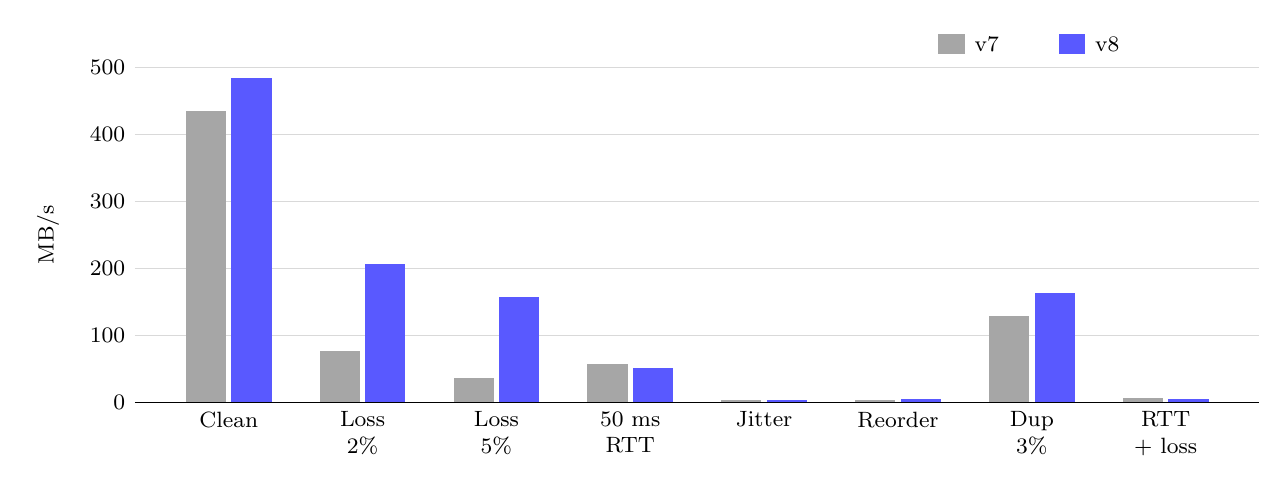
\begin{tikzpicture}[x=1.7cm,y=0.0085cm,font=\footnotesize]
  \foreach \y in {0,100,200,300,400,500} {\draw[black!15] (0.3,\y) -- (8.7,\y); \node[left] at (0.3,\y) {\y};}
  \foreach \i/\n/\a/\b in {1/Clean/435.4/483.6,2/Loss\\2\%/75.6/206.8,3/Loss\\5\%/36.0/157.3,4/50 ms\\RTT/57.5/51.4,
                           5/Jitter/2.7/2.8,6/Reorder/3.8/4.1,7/Dup\\3\%/128.6/163.1,8/RTT\\+ loss/6.8/5.2} {
    \fill[black!35] (\i-0.32,0) rectangle (\i-0.02,\a);
    \fill[blue!65] (\i+0.02,0) rectangle (\i+0.32,\b);
    \node[below,align=center] at (\i,0) {\n};
  }
  \draw (0.3,0) -- (8.7,0);
  \node[rotate=90] at (-0.35,250) {MB/s};
  \fill[black!35] (6.3,520) rectangle ++(0.2,30); \node[right] at (6.5,535) {v7};
  \fill[blue!65] (7.2,520) rectangle ++(0.2,30); \node[right] at (7.4,535) {v8};
\end{tikzpicture}}
\caption{Table~\ref{tab:netem} as a chart. The largest gains are under packet loss.}\label{fig:netem}
\end{figure}

\paragraph{Loss.} Version~8 gains most under loss: 2.7 times faster at 2\% and 4.4 times at 5\%. Selective
acknowledgement stops the resending of blocks the receiver already holds, and the timeout repairs a burst of
known holes at once instead of one block per timeout. The number of retransmissions stays roughly the same
(about 700 at 2\%, 1,700 at 5\%), but they are now the right ones.

\paragraph{Duplication.} Under duplication, version~8 makes no retransmissions at all, against 47 in version~7,
because duplicates no longer disturb the loss signal.

\paragraph{Jitter and reordering.} These are essentially unchanged. Both versions correctly treat a late block
as late rather than lost until the reorder delay expires, and at these settings the relay's own reordering
dominates.

\paragraph{Long delay.} With or without loss, version~8 is 11--24\% slower. This is the intended consequence of
fix~\#8. Version~7's window counted blocks of whatever size they had grown to, so it silently held up to 13
times more bytes than its nominal size. That inflated throughput on a clean long path, but it is unfair to
competing traffic and fragile under loss. Version~8 must earn its window through slow start and additive
increase. On transfers of 32~MiB the window does not reach the path's capacity, while longer transfers amortise
the ramp.

\section{Loopback throughput}

With 512~MiB over four lanes (median of three runs), version~7 reached 1,045~MB/s with 1,644 retransmissions and
version~8 1,079~MB/s with 706 retransmissions. The hardening therefore cost no loopback throughput, even though
every acknowledgement is now processed selectively. Flow control and selective acknowledgement more than halve
the needless retransmissions, which on loopback come from the receiver's rings overflowing, not from the
network.

\section{Earlier comparative benchmarks}

The repository's benchmark record~\cite{repo}, measured during development of versions~5--7 on a 16-core host,
compares Fuse with the quinn QUIC implementation~\cite{quinn}:
\begin{itemize}
  \item \textbf{File transfer.} For a 1~GiB file with both sides encrypted, Fuse reached 3,560~MB/s against
    1,947~MB/s for QUIC at four lanes, 1.8 times faster; unencrypted it was 1.3--2.2 times faster.
  \item \textbf{Latency under load.} Small-message 99th-percentile latency was 39.6~\textmu s alone and
    38.2~\textmu s while 6.3~GB/s of bulk traffic shared the session. A single QUIC connection carrying both
    inflated its tail latency 82 times; a second QUIC connection recovered most of it. This is the clearest
    evidence for per-stream congestion control.
\end{itemize}
These numbers were measured on loopback, with 16~KiB blocks that a 1,500-byte path would not allow, and compare
PSK encryption without forward secrecy against TLS~1.3 with it. They should be read as evidence about
mechanisms, not as predictions for a wide-area network.

\section{Threats to validity}

\begin{itemize}
  \item All measurements are single-host: impairments are emulated by a user-space relay, and no physical
    two-host or real 1,500-MTU path has been measured yet.
  \item Each cell of Table~\ref{tab:netem} is a single run; differences of a few percent are within noise.
  \item The relay itself limits absolute throughput at high rates, although it limits both versions equally.
  \item The comparison with QUIC predates version~8 and has not been repeated since.
\end{itemize}

\chapter{Limitations, Future Work and Conclusion}\label{ch:conclusion}

\section{Limitations}

\subsection{Open issues in the SDK and the HTTP mapping}

The socket-style SDK and the HTTP mapping were deliberately left out of the version~8 pass, which concentrated
on the protocol core. Their open findings are listed in Table~\ref{tab:open}. The first item in the table is
the most serious: an application that uses the SDK with encryption is still exposed to the GCM authentication-key
recovery described in Section~\ref{sec:nonce}, and fixing the SDK is the first item of future work.

\begin{table}[H]
\centering\small
\caption{Findings still open in the SDK and the HTTP mapping.}\label{tab:open}
\begin{tabularx}{\linewidth}{c>{\raggedright\arraybackslash}X}
\toprule
\textbf{\#} & \textbf{Issue} \\
\midrule
1 & SDK retransmissions re-seal with the retransmission bit in the AAD: the GCM nonce-reuse flaw remains in the SDK \\
2, 3 & SDK control messages are unauthenticated, and the SDK re-anchors its peer on any ACK, NACK or CLOSE \\
4 & The SDK server never authenticates the client, and allocates a connection, a socket and a thread per HELLO \\
12 & Idle SDK connections have no liveness check (HEARTBEAT is never sent) \\
13 & The SDK is stop-and-wait per message: only one message is in flight per direction \\
26 & About 17~MB per SDK connection: registry slots embed 16~KiB payloads while the SDK sends 1,200-byte blocks \\
27 & \code{fuse_close} frees the connection after two seconds even if a caller is still inside a call \\
28 & \code{fuse_connect} takes the PSK through \code{strlen}, so a key containing a zero byte is truncated \\
29 & HTTP: header injection (no CR/LF validation), timeout scope, reason truncation, detached threads, server status, and no tests \\
\bottomrule
\end{tabularx}
\end{table}

\subsection{Limitations of the protocol core}

\begin{itemize}
  \item \textbf{Fairness between lanes.} Every lane runs its own congestion controller, so a transfer with $N$
    lanes competes with other traffic on a shared bottleneck like $N$ TCP flows. Per-stream congestion control
    is the premise of the design, and it is what keeps a bulk stream from inflating the latency of a small one.
    The flip side is that a bulk transfer's \emph{aggregate} share should probably be coupled across its lanes.
  \item \textbf{Consecutive ports.} Bulk-transfer lanes need $N$ consecutive open UDP ports. A single-port
    transfer requires reworking the receive pipeline to demultiplex lanes by stream identifier on one socket.
  \item \textbf{Stragglers.} Static sharding means the slowest lane decides when the transfer completes; under
    heavy loss one lane can lag behind the others. Dynamic re-sharding or work stealing between lanes would
    address this.
  \item \textbf{Stage~4 flags are not exposed.} Unreliable, unordered and coalescing streams exist as tested
    primitives, and \code{fuse_bench} exercises a mixed session. No public transport offers them yet, so the
    mixed loss-tolerant and loss-intolerant session that motivates the protocol is not yet available to
    applications.
  \item \textbf{Forward secrecy and passwords.} The PSK path provides no forward secrecy. The DTLS~1.2 ECDHE-PSK
    component that would provide it is not wired into any transport. Accepting human-chosen passwords safely
    would need a PAKE such as CPace.
  \item \textbf{The multiplexed transfer} has no encryption, and therefore no control-plane authentication, and
    no address validation.
  \item \textbf{Platforms.} macOS uses one system call per datagram and cannot query the path MTU, so blocks do
    not grow there.
  \item \textbf{Evaluation.} All measurements are on one host with emulated impairments. There is no physical
    two-host run and no run on a real 1,500-MTU path, and the QUIC comparison predates version~8.
\end{itemize}

\section{Future work}

In order of priority, the next steps are:
\begin{enumerate}
  \item \textbf{Apply the version~8 hardening to the SDK}, reusing the bulk transfer's components rather than
    re-implementing them:
    \begin{itemize}
      \item the AAD fix;
      \item control-plane GMAC;
      \item path validation;
      \item Retry-style client validation before allocating per-connection state;
      \item heartbeats;
      \item a pipelined window instead of stop-and-wait;
      \item registry slots sized to the block.
    \end{itemize}
  \item \textbf{Fix the HTTP mapping's input validation}, and add tests.
  \item \textbf{Expose per-stream flags in a public API}, so an application can open a loss-tolerant and a
    loss-intolerant stream in one session. This is the feature that motivates the protocol.
  \item \textbf{Make the bulk transfer use a single port}, demultiplexing by stream identifier, and add work
    stealing between lanes.
  \item \textbf{Offer a forward-secret mode} by wiring the existing DTLS ECDHE-PSK handshake into session key
    establishment, keeping the per-lane AEAD data path. Add a PAKE for password-based deployments.
  \item \textbf{Couple congestion control across the lanes of one transfer}, so that the transfer as a whole is
    fair to other flows while its streams remain isolated from one another.
  \item \textbf{Evaluate on real networks}: two physical hosts, a 1,500-MTU wide-area path, and a fresh QUIC
    comparison against version~8.
  \item \textbf{Add fuzz testing of the decoders.} Every decoder is a natural fuzzing target, and none is fuzzed
    today.
\end{enumerate}

\section{Conclusion}

Fuse demonstrates that a transport whose reliability, ordering and congestion control are properties of
individual streams can be built on UDP with modest code. Its central ingredients are:
\begin{itemize}
  \item a ring-indexed selective-acknowledgement window;
  \item reorder-tolerant negative acknowledgements;
  \item per-stream AIMD with slow start, RFC~6298 timers and pacing;
  \item batched UDP I/O;
  \item per-lane parallel AEAD.
\end{itemize}
Earlier measurements showed the latency benefit of per-stream congestion control under mixed load, and
throughput competitive with a mature QUIC implementation.

The security and correctness review of version~7 showed how easily a datagram protocol goes wrong in ways that
tests of the happy path never reveal:
\begin{itemize}
  \item an innocuous flag in the AAD turned every retransmission into a key-recovery oracle;
  \item a convenient address re-anchoring became a hijacking primitive;
  \item an unused bitmask cost a factor of four in throughput under loss.
\end{itemize}
Protocol version~8 fixes all of these in the protocol core, mostly by adopting mechanisms whose design rationale
is well established in QUIC and TCP: Retry tokens, path validation, AEAD usage limits, selective
acknowledgement, RFC~6298 timers, pacing and MTU discovery. It does so without any loss of loopback throughput,
and with large gains under loss. The remaining work, above all the SDK, is now well defined.


\appendix
\chapter{Configuration and Status Reference}\label{app:config}

\begin{table}[H]
\centering\small
\caption{\texttt{TransferConfig} fields (\texttt{fuse/transfer.hpp}).}\label{tab:config}
\begin{tabularx}{\linewidth}{>{\raggedright\arraybackslash}p{4.1cm}>{\raggedright\arraybackslash}p{2.6cm}X}
\toprule
\textbf{Field} & \textbf{Default} & \textbf{Meaning} \\
\midrule
\code{host}, \code{bind_address} & \code{127.0.0.1}, \code{0.0.0.0} & sender's destination; receiver's local address (IPv4 or IPv6) \\
\code{base_port} & 4433 & lane $i$ uses \code{base_port}$+i$; the range must end at or below 65,535 \\
\code{lanes} & 4 & parallel shards; throughput is not monotonic in lanes, so measure before raising \\
\code{block_size} & 1,200 & starting payload per block; grows on clean paths up to the route MTU \\
\code{pre_shared_key} & empty & non-empty enables AES-256-GCM; at least 16 random bytes \\
\code{timeout_ms} & 120,000 & give up after this long without progress \\
\code{connect_timeout_ms} & 10,000 & sender: give up reaching the receiver \\
\code{cancel} & null & pointer to an atomic flag; setting it aborts both ends promptly \\
\code{on_progress}, \code{progress_interval_ms} & none, 250 & progress callback, run on the caller's thread \\
\code{writer_threads}, \code{ring_slots} & 2, 256 & receive pipeline size (about 51~MB of rings with 4 lanes) \\
\code{resume_checkpoint_ms} & 1,000 & how often \code{receive_file} saves resume progress \\
\bottomrule
\end{tabularx}
\end{table}

\begin{table}[H]
\centering\small
\caption{\texttt{TransferStatus} values.}\label{tab:status}
\begin{tabularx}{\linewidth}{lX}
\toprule
\textbf{Status} & \textbf{Meaning} \\
\midrule
\code{Ok} & every byte delivered (and, for a resumed file, verified) \\
\code{ConfigError} & invalid configuration (no lanes, port range past 65,535, short PSK, \ldots) \\
\code{SocketError} & bind or socket failure \\
\code{Timeout} & peer silent, or no progress \\
\code{AuthFailed} & keys differ, or blocks failed authentication \\
\code{Incomplete} & finished short of the expected bytes \\
\code{Unsupported} & encryption requested from a build without cryptography \\
\code{ResourceLimit} & the peer's claimed size could not be allocated \\
\code{Cancelled}, \code{PeerAborted} & this side cancelled; the other side gave up and said so \\
\code{IoError} & the output could not be written \\
\code{VerifyFailed} & a resumed file did not match the sender's digest \\
\code{VersionMismatch} & the peer speaks a different protocol version \\
\bottomrule
\end{tabularx}
\end{table}

\chapter{Guide to the Repository}\label{app:files}

\begingroup\small
\begin{xltabular}{\linewidth}{>{\raggedright\arraybackslash}p{4.4cm}X}
\caption{Files of the protocol core and the transports.}\label{tab:files}\\
\toprule
\textbf{File} & \textbf{Responsibility and key entry points} \\
\midrule\endfirsthead
\toprule
\textbf{File} & \textbf{Responsibility and key entry points} \\
\midrule\endhead
\bottomrule\endfoot
\code{wire.hpp} & Protocol version, message types, size limits, big-endian helpers, extension helpers \\
\code{block.hpp/.cpp} & DATA codec, type dispatch (\code{peek_msg_type}), version-mismatch reply \\
\code{control.hpp/.cpp} & Every control message's structure and codec \\
\code{registry.hpp/.cpp} & Sender retransmit store; \code{apply_ack} \\
\code{receiver.hpp/.cpp} & Receive window, gap timing, \code{collect_nacks} \\
\code{congestion.hpp} & Per-stream AIMD, slow start, RTT and RTTVAR, RTO with backoff, pacing \\
\code{setup.hpp/.cpp} & SETUP codec, validation, initiator and responder state machines \\
\code{reassembly.hpp/.cpp} & Ordered and unordered delivery into a sink \\
\code{send_queue.hpp} & Coalescing or back-pressuring send queue \\
\code{spsc_ring.hpp} & Lock-free single-producer, single-consumer ring \\
\code{orchestrator.hpp/.cpp} & Autoscaling worker pool \\
\code{udp.hpp}, \code{udp_common.cpp}, \code{udp_linux.cpp}, \code{udp_darwin.cpp} & UDP socket, addresses, GSO send, batched receive, route MTU \\
\code{session_crypto.hpp/.cpp} & HKDF, AES-256-GCM lane cipher, key epochs, control GMAC, secure random numbers \\
\code{dtls.hpp/.cpp} & DTLS~1.2 ECDHE-PSK session (standalone) \\
\code{digest.hpp/.cpp} & Whole-file and segmented SHA-256 (FNV fallback) \\
\code{hash.hpp} & FNV-1a-64 and SipHash-2-4 \\
\code{transfer.hpp}, \code{transfer.cpp} & Bulk transfer: sharding, lane handshake with address validation, sender loop, receive pipeline, sinks, resume, cancellation, status ranking \\
\code{mux_transfer.hpp/.cpp} & Multiplexed transfer: SETUP, per-stream state, worker task, NACK backlog \\
\code{sdk.h}, \code{sdk.cpp} & Socket-style C API: HELLO/HELLO\_ACK, pump thread, message framing, close \\
\code{http.h}, \code{http.cpp} & One HTTP/1.1 exchange per SDK connection \\
\code{fuse.h}, \code{packet.h}, \code{varint.h}, \code{src/*.c} & Legacy C scaffold, unused by the protocol \\
\code{tests/proto/test_*.cpp} & One suite per component and transport \\
\code{bench/} & \code{fuse_bench}, \code{fuse_filebench} and the QUIC baseline, \code{fuse_latbench}, \code{fuse_netem}, \code{RESULTS.md} \\
\code{examples/} & Stage~1 sender and receiver demonstration; echo server and client \\
\code{scripts/}, \code{.github/workflows/} & Install and release scripts, network simulation; CI matrix and releases \\
\end{xltabular}
\endgroup

\chapter{Building and Reproducing the Results}\label{app:build}

\begin{lstlisting}[language=bash]
# Build and run the tests (wolfSSL is fetched automatically;
# add -DFUSE_WITH_CRYPTO=OFF for a faster build without encryption)
cmake --preset default
cmake --build --preset default
ctest --preset default -j8

# Stage 1 demonstration: block 3 is dropped once and recovered by a NACK
./build/default/examples/fuse_stage1_receiver 48000 &
./build/default/examples/fuse_stage1_sender 127.0.0.1 48000 --drop 3 --count 8

# A transfer through the network emulator: 4 lanes, 12 ms one-way delay, 1% loss
./build/default/bench/fuse_netem 46000 4 127.0.0.1 45000 --delay-ms 12 --loss-pct 1 &
#   receiver uses base_port 45000, sender uses base_port 46000 (see bench/README.md)
\end{lstlisting}

\chapter{Glossary}\label{app:glossary}

\begin{description}[leftmargin=2.6cm,labelwidth=2.4cm,style=sameline,itemsep=1pt]
  \item[AAD] Additional authenticated data: input to an AEAD that is authenticated but not encrypted.
  \item[AEAD] Authenticated encryption with associated data, here AES-256-GCM.
  \item[AIMD] Additive increase, multiplicative decrease: the congestion-control rule.
  \item[Base] The lowest sequence number not yet received (receiver) or acknowledged (sender).
  \item[Block] One DATA datagram, independently addressed and retransmittable.
  \item[Epoch] A run of $2^{22}$ sequence numbers that share one data key.
  \item[GMAC] GCM used with an empty plaintext, i.e.\ as a message authentication code.
  \item[GSO] Generic segmentation offload: one large UDP send split into datagrams by the kernel.
  \item[Lane] One shard of a bulk transfer: one port, one thread per side, one reliable stream.
  \item[NACK] Negative acknowledgement: an explicit list of missing sequence numbers.
  \item[PSK] Pre-shared key.
  \item[RTO] Retransmission timeout.
  \item[RTT, SRTT] Round-trip time; its smoothed estimate.
  \item[rwnd] The receive window advertised in ACKs, for flow control.
  \item[SACK] Selective acknowledgement: the ACK bitmask of blocks received above the base.
  \item[SPSC] Single producer, single consumer: the lock-free ring.
  \item[Stream] An independent sequence-numbered flow (SDK and multiplexed transfer); a lane in the bulk transfer.
  \item[Token] The address-validation value a receiver issues in a Retry and expects back in the StreamStart.
\end{description}


\begin{thebibliography}{99}
\addcontentsline{toc}{chapter}{References}

\bibitem{rfc9000} J.~Iyengar and M.~Thomson, ``QUIC: A UDP-Based Multiplexed and Secure Transport,'' RFC~9000, IETF, May 2021.

\bibitem{rfc9001} M.~Thomson and S.~Turner, ``Using TLS to Secure QUIC,'' RFC~9001, IETF, May 2021. (\S6.6: AEAD usage limits.)

\bibitem{rfc9002} J.~Iyengar and I.~Swett, ``QUIC Loss Detection and Congestion Control,'' RFC~9002, IETF, May 2021.

\bibitem{rfc9293} W.~Eddy (Ed.), ``Transmission Control Protocol (TCP),'' RFC~9293, IETF, Aug.\ 2022.

\bibitem{rfc5681} M.~Allman, V.~Paxson and E.~Blanton, ``TCP Congestion Control,'' RFC~5681, IETF, Sep.\ 2009.

\bibitem{rfc2018} M.~Mathis, J.~Mahdavi, S.~Floyd and A.~Romanow, ``TCP Selective Acknowledgment Options,'' RFC~2018, IETF, Oct.\ 1996.

\bibitem{rfc6298} V.~Paxson, M.~Allman, J.~Chu and M.~Sargent, ``Computing TCP's Retransmission Timer,'' RFC~6298, IETF, Jun.\ 2011.

\bibitem{rfc7323} D.~Borman, B.~Braden, V.~Jacobson and R.~Scheffenegger, ``TCP Extensions for High Performance,'' RFC~7323, IETF, Sep.\ 2014.

\bibitem{rfc8899} G.~Fairhurst, T.~Jones, M.~T\"uxen, I.~R\"ungeler and T.~V\"olker, ``Packetization Layer Path MTU Discovery for Datagram Transports,'' RFC~8899, IETF, Sep.\ 2020.

\bibitem{rfc5869} H.~Krawczyk and P.~Eronen, ``HMAC-based Extract-and-Expand Key Derivation Function (HKDF),'' RFC~5869, IETF, May 2010.

\bibitem{rfc8446} E.~Rescorla, ``The Transport Layer Security (TLS) Protocol Version 1.3,'' RFC~8446, IETF, Aug.\ 2018.

\bibitem{rfc6347} E.~Rescorla and N.~Modadugu, ``Datagram Transport Layer Security Version 1.2,'' RFC~6347, IETF, Jan.\ 2012.

\bibitem{rfc9147} E.~Rescorla, H.~Tschofenig and N.~Modadugu, ``The Datagram Transport Layer Security (DTLS) Protocol Version 1.3,'' RFC~9147, IETF, Apr.\ 2022.

\bibitem{rfc4279} P.~Eronen and H.~Tschofenig, ``Pre-Shared Key Ciphersuites for Transport Layer Security (TLS),'' RFC~4279, IETF, Dec.\ 2005.

\bibitem{rfc1350} K.~Sollins, ``The TFTP Protocol (Revision 2),'' RFC~1350, IETF, Jul.\ 1992.

\bibitem{rfc8085} L.~Eggert, G.~Fairhurst and G.~Shepherd, ``UDP Usage Guidelines,'' RFC~8085, IETF, Mar.\ 2017.

\bibitem{rfc7838} M.~Nottingham, P.~McManus and J.~Reschke, ``HTTP Alternative Services,'' RFC~7838, IETF, Apr.\ 2016.

\bibitem{nist-gcm} M.~Dworkin, ``Recommendation for Block Cipher Modes of Operation: Galois/Counter Mode (GCM) and GMAC,'' NIST Special Publication 800-38D, Nov.\ 2007.

\bibitem{joux} A.~Joux, ``Authentication Failures in NIST version of GCM,'' comments submitted to NIST, 2006.

\bibitem{siphash} J.-P.~Aumasson and D.~J.~Bernstein, ``SipHash: a fast short-input PRF,'' in \emph{Progress in Cryptology -- INDOCRYPT 2012}, LNCS 7668, Springer, 2012, pp.~489--508.

\bibitem{jacobson} V.~Jacobson, ``Congestion Avoidance and Control,'' in \emph{Proc.\ ACM SIGCOMM '88}, 1988, pp.~314--329.

\bibitem{mathis} M.~Mathis, J.~Semke, J.~Mahdavi and T.~Ott, ``The Macroscopic Behavior of the TCP Congestion Avoidance Algorithm,'' \emph{ACM SIGCOMM Computer Communication Review}, vol.~27, no.~3, pp.~67--82, 1997.

\bibitem{chiu-jain} D.-M.~Chiu and R.~Jain, ``Analysis of the Increase and Decrease Algorithms for Congestion Avoidance in Computer Networks,'' \emph{Computer Networks and ISDN Systems}, vol.~17, no.~1, pp.~1--14, 1989.

\bibitem{quic-design} A.~Langley et~al., ``The QUIC Transport Protocol: Design and Internet-Scale Deployment,'' in \emph{Proc.\ ACM SIGCOMM '17}, 2017, pp.~183--196.

\bibitem{sctp} R.~Stewart (Ed.), ``Stream Control Transmission Protocol,'' RFC~9260, IETF, Jun.\ 2022.

\bibitem{udt} Y.~Gu and R.~L.~Grossman, ``UDT: UDP-based data transfer for high-speed wide area networks,'' \emph{Computer Networks}, vol.~51, no.~7, pp.~1777--1799, 2007.

\bibitem{gso} W.~de~Bruijn and E.~Dumazet, ``Optimizing UDP for content delivery: GSO, pacing and zerocopy,'' Linux Plumbers Conference, 2018; Linux kernel \texttt{UDP\_SEGMENT} socket option (since 4.18).

\bibitem{recvmmsg} Linux man-pages project, \texttt{recvmmsg(2)} and \texttt{sendmmsg(2)}.

\bibitem{netem} S.~Hemminger, ``Network Emulation with NetEm,'' in \emph{Proc.\ Linux Conf Australia}, 2005; Linux \texttt{tc-netem(8)} manual.

\bibitem{lamport-spsc} L.~Lamport, ``Specifying Concurrent Program Modules,'' \emph{ACM Transactions on Programming Languages and Systems}, vol.~5, no.~2, pp.~190--222, 1983. (The single-producer/single-consumer ring.)

\bibitem{wolfssl} wolfSSL Inc., \emph{wolfSSL / wolfCrypt Embedded SSL/TLS Library}, \url{https://www.wolfssl.com/}.

\bibitem{quinn} The quinn project, \emph{quinn: async-friendly QUIC implementation in Rust}, \url{https://github.com/quinn-rs/quinn}.

\bibitem{fnv} G.~Fowler, L.~C.~Noll, K.-P.~Vo, D.~Eastlake and T.~Hansen, ``The FNV Non-Cryptographic Hash Algorithm,'' IETF Internet-Draft draft-eastlake-fnv.

\bibitem{repo} Fuse project repository, \code{kamalkoushikd/fuse-nw}: \code{docs/PROTOCOL.md} (wire protocol, version 8), \code{docs/ROADMAP.md} (status and review findings), \code{bench/RESULTS.md} (benchmarks).

\end{thebibliography}


\end{document}
